\documentclass[
  10pt,
  aspectratio=169,
  utf8,
  xcolor={dvipsnames}
]{beamer}

\usetheme[
  progressbar=foot,
  sectionpage=progressbar,
  subsectionpage=progressbar,
  numbering=fraction
]{metropolis}
\usefonttheme{metropolis}
\usecolortheme{spruce}
\setbeamercolor{progress bar}{fg=MidnightBlue, bg=LightSteelBlue}
\setbeamercolor{title}{fg=MidnightBlue}
\setbeamercolor{frame title}{fg=MidnightBlue}
\setbeamercolor{structure}{fg=MidnightBlue}

\usepackage{booktabs}
\usepackage{graphicx}
\usepackage{tikz}
\usetikzlibrary{shapes, arrows, positioning, fit, backgrounds}
\usepackage{amsmath}
\usepackage{fontspec}
\usepackage{caption}
\captionsetup[figure]{labelformat=empty}
\captionsetup[table]{labelformat=empty}

\title{\textbf{Health Informatics: Contemporary Challenges and Applications in Global Health Systems}}
\subtitle{MSc Public Health Data Science - SDS6210 Informatics for Health}
\author{\textbf{Cavin Otieno}}
\institute{Department of Public Health\\University}
\date{\today}

\begin{document}

% Group Members Frame
{
\setbeamertemplate{footline}{}
\begin{frame}
\titlepage
\end{frame}
}

\begin{frame}{Group 5 Members}
\begin{center}
\begin{tabular}{ll}
\toprule
\textbf{Student ID} & \textbf{Student Name} \\
\midrule
SDS6/46982/2024 & Cavin Otieno \\
SDS6/47543/2024 & Laura Nabalayo Kundu \\
SDS6/47659/2024 & John Andrew \\
\bottomrule
\end{tabular}
\end{center}
\end{frame}

\begin{frame}{Table of Contents}
\tableofcontents
\end{frame}

\section{Module Overview: Health Informatics in Context}

\begin{frame}{Learning Objectives}
This comprehensive presentation addresses four critical domains in health informatics:

\begin{itemize}
\item \textbf{Electronic Health Records (EHRs)} in resource-constrained settings
\item \textbf{Health Informatics} and its contribution to Universal Health Coverage (UHC)
\item \textbf{Digital Transformation} and its impact on patient-centered care
\item \textbf{Interoperability} challenges in national health information systems
\end{itemize}

Each section applies systems-thinking frameworks and evidence-based analysis appropriate for MSc-level evaluation.
\end{frame}

\begin{frame}{Conceptual Framework: Health Systems Perspective}
\begin{center}
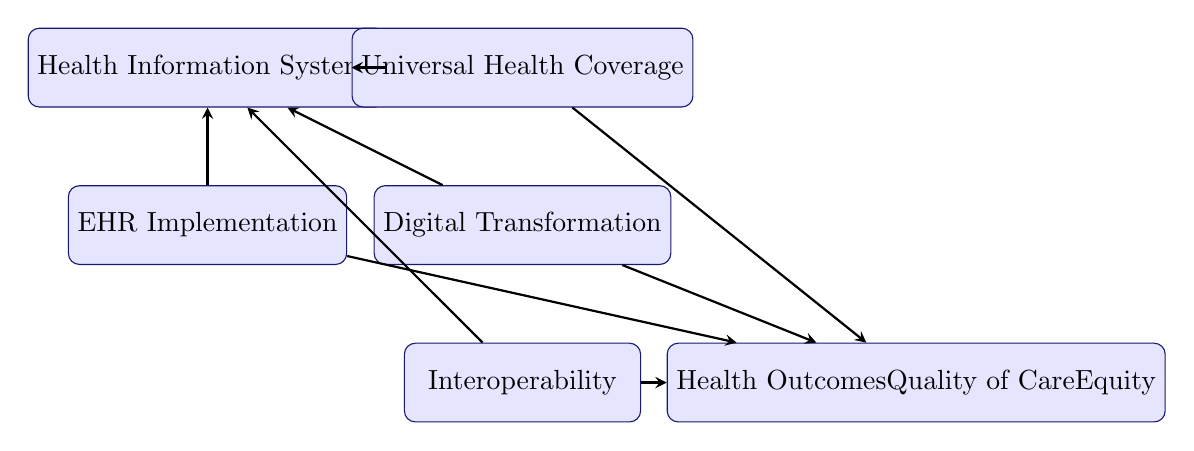
\begin{tikzpicture}[node distance=2cm]
\tikzstyle{block} = [rectangle, rounded corners, minimum width=3cm, minimum height=1cm, text centered, draw=MidnightBlue, fill=blue!10]
\tikzstyle{arrow} = [thick,->,>=stealth]

\node (HIS) [block] {Health Information Systems};
\node (EHRS) [block, below of=HIS] {EHR Implementation};
\node (UHC) [block, right of=HIS, xshift=2cm] {Universal Health Coverage};
\node (DTC) [block, below of=UHC] {Digital Transformation};
\node (INT) [block, below of=DTC] {Interoperability};

\draw [arrow] (HIS) -- (UHC);
\draw [arrow] (EHRS) -- (HIS);
\draw [arrow] (DTC) -- (HIS);
\draw [arrow] (INT) -- (HIS);

\node (OUTCOMES) [block, right of=INT, xshift=3cm] {Health Outcomes\\Quality of Care\\Equity};
\draw [arrow] (UHC) -- (OUTCOMES);
\draw [arrow] (DTC) -- (OUTCOMES);
\draw [arrow] (INT) -- (OUTCOMES);
\draw [arrow] (EHRS) -- (OUTCOMES);
\end{tikzpicture}
\end{center}
\end{frame}

% ============================================================================
% SECTION 1: ELECTRONIC HEALTH RECORDS IN RESOURCE-CONSTRAINED SETTINGS
% ============================================================================

\section{EHRs in Rural and Resource-Constrained Settings}

\subsection{Definitions and Conceptual Foundations}

\begin{frame}{Electronic Health Records: Definition}
According to the World Health Organization (2016), an Electronic Health Record (EHR) is:

\begin{block}{WHO Definition}
"A longitudinal electronic record of patient health information generated by one or more encounters in any care delivery setting, including patient demographics, progress notes, problems, medications, vital signs, past medical history, immunizations, laboratory data, and radiology reports."
\end{block}

Key characteristics that distinguish EHRs from basic electronic records:
\begin{itemize}
\item \textbf{Interoperability} - Ability to exchange information across systems
\item \textbf{Decision support} - Clinical alerts, reminders, and evidence-based guidance
\item \textbf{Patient-centered} - Comprehensive view of patient health history
\item \textbf{Longitudinal} - Captures health data across time and care episodes
\end{itemize}
\end{frame}

\begin{frame}{The Role of EHRs in Health Systems}
EHRs serve multiple functions within the WHO health systems framework:

\begin{columns}
\begin{column}{0.5\textwidth}
\begin{block}{Service Delivery}
\begin{itemize}
\item Clinical documentation
\item Care coordination
\item Referral management
\end{itemize}
\end{block}
\begin{block}{Health Information}
\begin{itemize}
\item Population health surveillance
\item Disease registries
\item Quality indicators
\end{itemize}
\end{block}
\end{column}
\begin{column}{0.5\textwidth}
\begin{block}{Medical Products}
\begin{itemize}
\item Medication reconciliation
\item Pharmacy integration
\end{itemize}
\end{block}
\begin{block}{Financing}
\begin{itemize}
\item Claims processing
\item Resource allocation
\end{itemize}
\end{block}
\end{column}
\end{columns}
\end{frame}

\subsection{Challenges: Infrastructure and Connectivity}

\begin{frame}{Infrastructure Challenges}
\begin{center}
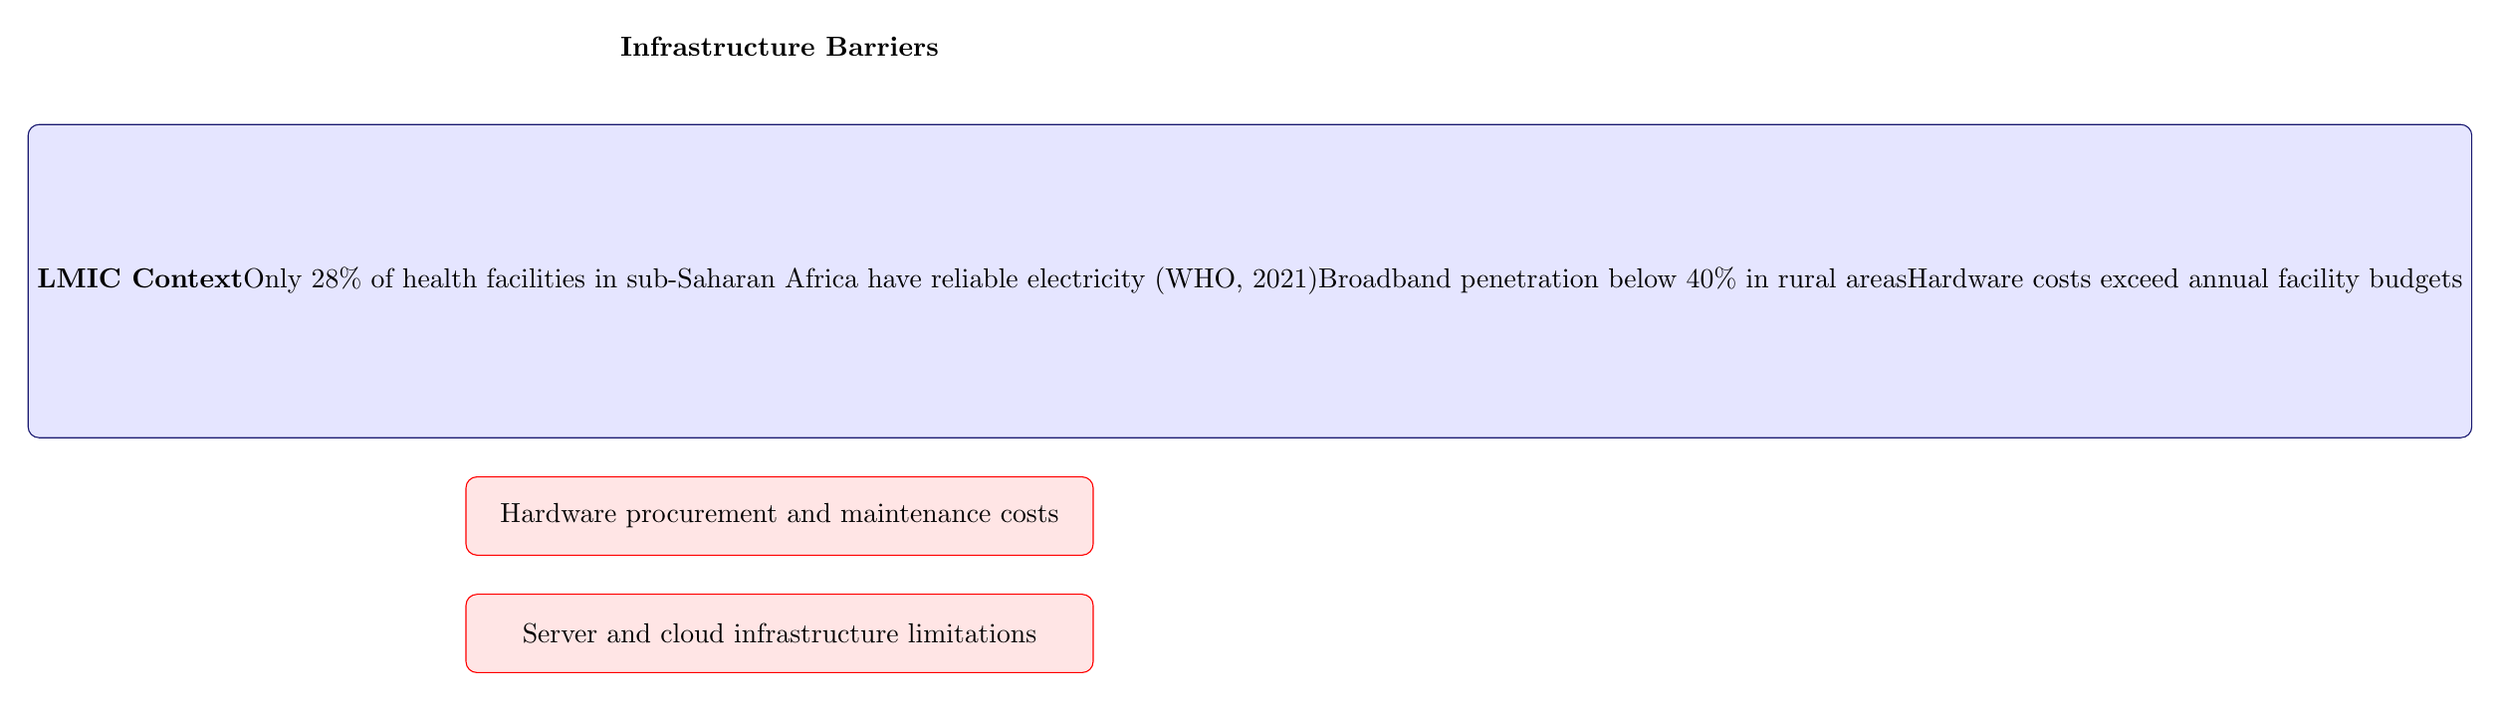
\begin{tikzpicture}[node distance=1.5cm]
\tikzstyle{challenge} = [rectangle, minimum width=8cm, minimum height=1cm, text centered, draw=Red, fill=red!10, rounded corners]
\tikzstyle{arrow} = [thick,->,>=stealth]

\node (title) at (0,3) {\textbf{Infrastructure Barriers}};
\node (grid) [challenge] {Unreliable electricity supply};
\node (net) [challenge, below of=grid] {Limited internet connectivity};
\node (hard) [challenge, below of=net] {Hardware procurement and maintenance costs};
\node (server) [challenge, below of=hard] {Server and cloud infrastructure limitations};

\node (context) at (6,0) [rectangle, rounded corners, draw=MidnightBlue, fill=blue!10, minimum width=4cm, minimum height=4cm]
{\textbf{LMIC Context}\\[0.3cm]Only 28\% of health facilities in sub-Saharan Africa have reliable electricity (WHO, 2021)\\Broadband penetration below 40\% in rural areas\\Hardware costs exceed annual facility budgets};
\end{tikzpicture}
\end{center}
\end{frame}

\begin{frame}{Case Study: EHR Implementation in Kenya}
The Kenyan Health Information System (KHIS) experience illustrates infrastructure challenges:

\begin{itemize}
\item \textbf{Power Supply}: 67\% of primary health facilities experience daily power outages
\item \textbf{Connectivity}: Only 34\% of rural facilities have reliable internet for DHIS2 synchronization
\item \textbf{Hardware Age}: Average computer age in public facilities exceeds 7 years
\end{itemize}

\begin{block}{Key Insight}
The digital health infrastructure gap represents the most fundamental barrier to EHR adoption in LMICs, with cascade effects on all other implementation components.
\end{block}
\end{frame}

\subsection{Challenges: Human Resources and Digital Skills}

\begin{frame}{Human Resource Constraints}
\begin{center}
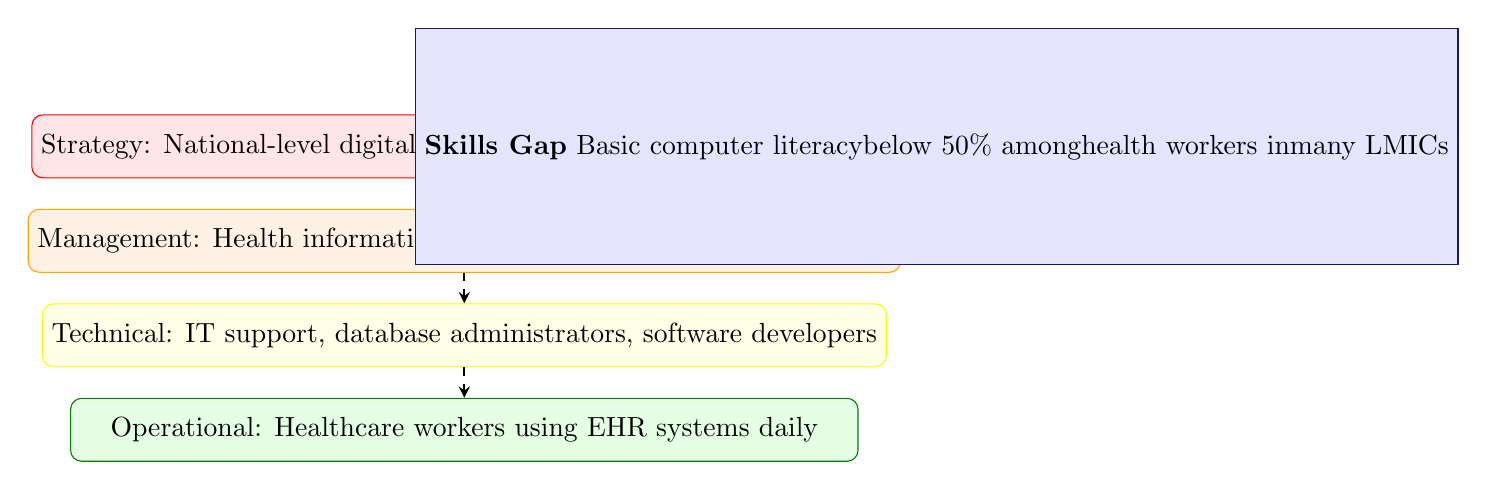
\begin{tikzpicture}[node distance=1.2cm]
\tikzstyle{level} = [rectangle, rounded corners, minimum width=10cm, minimum height=0.8cm, text centered]
\tikzstyle{arrow} = [thick,->,>=stealth]

\node (L1) [level, draw=Red, fill=red!10] {Strategy: National-level digital health policy and governance capacity};
\node (L2) [level, below of=L1, draw=Orange, fill=orange!10] {Management: Health informatics managers and system administrators};
\node (L3) [level, below of=L2, draw=Yellow, fill=yellow!10] {Technical: IT support, database administrators, software developers};
\node (L4) [level, below of=L3, draw=Green, fill=green!10] {Operational: Healthcare workers using EHR systems daily};

\draw [arrow, dashed] (L1) -- (L2);
\draw [arrow, dashed] (L2) -- (L3);
\draw [arrow, dashed] (L3) -- (L4);

\node (gap) at (6,0) [rectangle, draw=MidnightBlue, fill=blue!10, minimum width=4cm, minimum height=3cm]
{\textbf{Skills Gap}\\[0.2cm]
Basic computer literacy\\below 50\% among\\health workers in\\many LMICs};
\end{tikzpicture}
\end{center}
\end{frame}

\begin{frame}{Task-Shifting and Training Models}
Evidence from LMICs supports task-shifting approaches:

\begin{columns}
\begin{column}{0.5\textwidth}
\begin{block}{Successful Models}
\begin{itemize}
\item Community health workers as data entry personnel
\item Dedicated health records officers
\item Peer mentorship programs
\end{itemize}
\end{block}
\end{column}
\begin{column}{0.5\textwidth}
\begin{block}{Training Challenges}
\begin{itemize}
\item High staff turnover (30-50\% annually)
\item Limited training resources
\item Resistance to workflow changes
\end{itemize}
\end{block}
\end{column}
\end{columns}

\begin{block}{Key Challenge}
The WHO estimates a global deficit of 18 million health workers, with the most acute shortages in regions requiring EHR implementation.
\end{block}
\end{frame}

\subsection{Challenges: Financial and Sustainability}

\begin{frame}{Financial Sustainability Framework}
\begin{center}
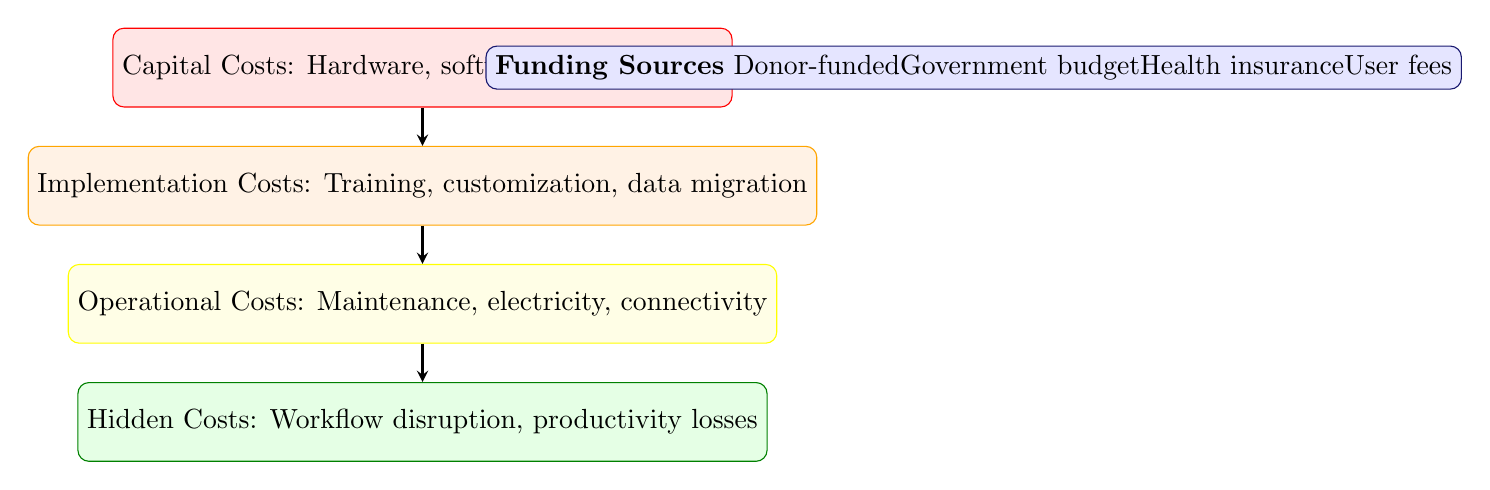
\begin{tikzpicture}[node distance=1.5cm]
\tikzstyle{cost} = [rectangle, rounded corners, minimum width=7cm, minimum height=1cm, text centered]
\tikzstyle{arrow} = [thick,->,>=stealth]

\node (C1) [cost, draw=Red, fill=red!10] {Capital Costs: Hardware, software, infrastructure};
\node (C2) [cost, below of=C1, draw=Orange, fill=orange!10] {Implementation Costs: Training, customization, data migration};
\node (C3) [cost, below of=C2, draw=Yellow, fill=yellow!10] {Operational Costs: Maintenance, electricity, connectivity};
\node (C4) [cost, below of=C3, draw=Green, fill=green!10] {Hidden Costs: Workflow disruption, productivity losses};

\draw [arrow] (C1) -- (C2);
\draw [arrow] (C2) -- (C3);
\draw [arrow] (C3) -- (C4);

\node (funding) at (7,0) [rectangle, rounded corners, draw=MidnightBlue, fill=blue!10, minimum width=4cm]
{\textbf{Funding Sources}\\[0.2cm]
Donor-funded\\Government budget\\Health insurance\\User fees};
\end{tikzpicture}
\end{center}
\end{frame}

\begin{frame}{Cost-Benefit Analysis Considerations}
Evidence on EHR cost-effectiveness in LMICs remains limited:

\begin{block}{Potential Benefits}
\begin{itemize}
\item Reduced paper storage costs
\item Improved medication safety
\item Better resource utilization data
\end{itemize}
\end{block}

\begin{block}{Implementation Realities}
\begin{itemize}
\item Total cost of ownership often underestimated by 200-300\%
\item Benefits typically realized after 3-5 years
\item Sustainability depends on domestic funding transitions
\end{itemize}
\end{block}

\begin{block}{Critical Finding}
The average EHR implementation in sub-Saharan Africa costs \$15,000-\$50,000 per facility, with annual operational costs representing 20-30\% of initial investment.
\end{block}
\end{frame}

\subsection{Challenges: Data Quality, Security, and Privacy}

\begin{frame}{Data Quality Dimensions}
\begin{center}
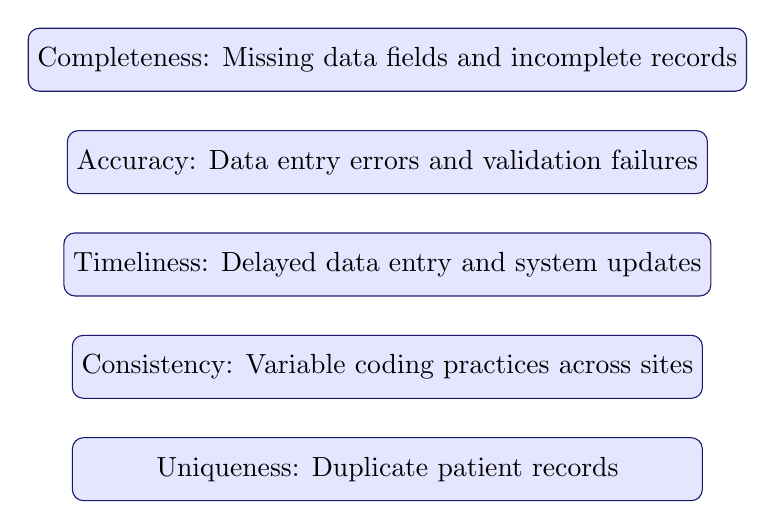
\begin{tikzpicture}[node distance=1.3cm]
\tikzstyle{dim} = [rectangle, rounded corners, minimum width=8cm, minimum height=0.8cm, text centered]

\node (D1) [dim, draw=MidnightBlue, fill=blue!10] {Completeness: Missing data fields and incomplete records};
\node (D2) [dim, below of=D1, draw=MidnightBlue, fill=blue!10] {Accuracy: Data entry errors and validation failures};
\node (D3) [dim, below of=D2, draw=MidnightBlue, fill=blue!10] {Timeliness: Delayed data entry and system updates};
\node (D4) [dim, below of=D3, draw=MidnightBlue, fill=blue!10] {Consistency: Variable coding practices across sites};
\node (D5) [dim, below of=D4, draw=MidnightBlue, fill=blue!10] {Uniqueness: Duplicate patient records};
\end{tikzpicture}
\end{center}
\end{frame}

\begin{frame}{Data Security and Privacy Concerns}
Data protection challenges in resource-constrained settings:

\begin{columns}
\begin{column}{0.5\textwidth}
\begin{block}{Security Threats}
\begin{itemize}
\item Physical theft of hardware
\item Malware and ransomware
\item Unauthorized network access
\end{itemize}
\end{block}
\end{column}
\begin{column}{0.5\textwidth}
\begin{block}{Privacy Concerns}
\begin{itemize}
\item Consent management challenges
\item Data sharing without authorization
\item Limited audit capabilities
\end{itemize}
\end{block}
\end{column}
\end{columns}

\begin{block}{Regulatory Environment}
Most LMICs lack comprehensive data protection legislation, creating legal uncertainty for EHR implementers and potential risks for patient privacy.
\end{block}
\end{frame}

\subsection{Challenges: Governance, Policy, and Sociocultural Factors}

\begin{frame}{Governance and Policy Gaps}
\begin{center}
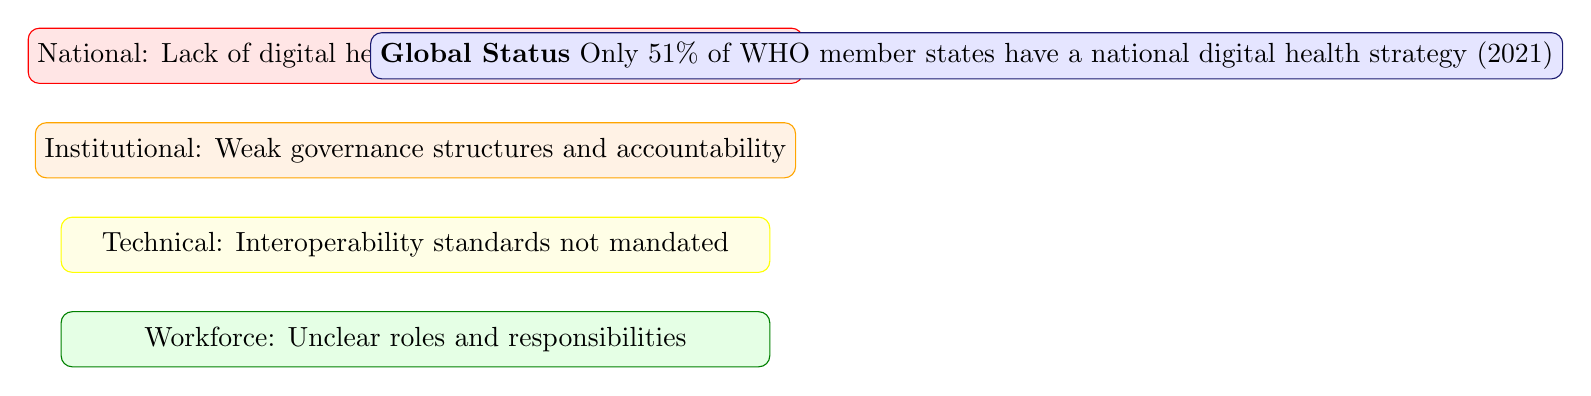
\begin{tikzpicture}[node distance=1.2cm]
\tikzstyle{level} = [rectangle, rounded corners, minimum width=9cm, minimum height=0.7cm, text centered]
\tikzstyle{arrow} = [thick,->,>=stealth]

\node (P1) [level, draw=Red, fill=red!10] {National: Lack of digital health strategies and EHR standards};
\node (P2) [level, below of=P1, draw=Orange, fill=orange!10] {Institutional: Weak governance structures and accountability};
\node (P3) [level, below of=P2, draw=Yellow, fill=yellow!10] {Technical: Interoperability standards not mandated};
\node (P4) [level, below of=P3, draw=Green, fill=green!10] {Workforce: Unclear roles and responsibilities};

\node (status) at (7,0) [rectangle, rounded corners, draw=MidnightBlue, fill=blue!10, minimum width=4cm]
{\textbf{Global Status}\\[0.2cm]
Only 51\% of WHO member states have a national digital health strategy (2021)};
\end{tikzpicture}
\end{center}
\end{frame}

\begin{frame}{Sociocultural and Organizational Barriers}
\begin{columns}
\begin{column}{0.5\textwidth}
\begin{block}{Sociocultural Factors}
\begin{itemize}
\item Resistance to technology adoption
\item Trust concerns about data use
\item Literacy and language barriers
\end{itemize}
\end{block}
\end{column}
\begin{column}{0.5\textwidth}
\begin{block}{Organizational Factors}
\begin{itemize}
\item Hierarchical decision-making cultures
\item Change management challenges
\item Competing priorities and workload
\end{itemize}
\end{block}
\end{column}
\end{columns}

\begin{block}{Case Example: South Africa}
The National Health Act (2003) provides a legal framework for health information, but implementation has been slow due to resource constraints, organizational resistance, and fragmented governance of digital health initiatives.
\end{block}
\end{frame}

\subsection{Systems Analysis: Causal Loop Diagram}

\begin{frame}{Systems Dynamics: EHR Implementation}
\begin{center}
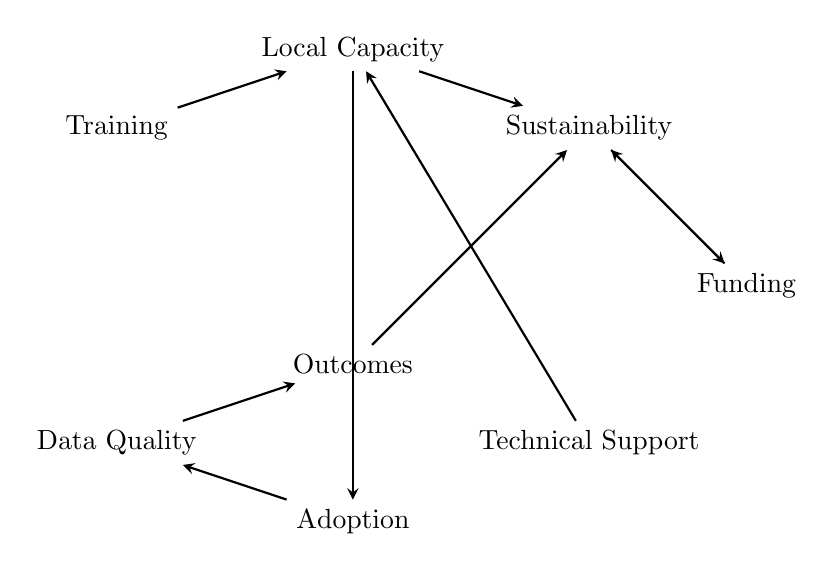
\begin{tikzpicture}[node distance=2cm]
\tikzstyle{node} = [circle, draw=MidnightBlue, fill=blue!20, minimum size=1cm]
\tikzstyle{arrow} = [thick,->,>=stealth]

\node (training) at (-3,2) {Training};
\node (capacity) at (0,3) {Local Capacity};
\node (sustain) at (3,2) {Sustainability};
\node (funding) at (5,0) {Funding};
\node (support) at (3,-2) {Technical Support};
\node (adoption) at (0,-3) {Adoption};
\node (data) at (-3,-2) {Data Quality};
\node (outcomes) at (0,-1) {Outcomes};

\draw [arrow] (training) -- (capacity);
\draw [arrow] (capacity) -- (sustain);
\draw [arrow] (funding) -- (sustain);
\draw [arrow] (support) -- (capacity);
\draw [arrow] (sustain) -- (funding);
\draw [arrow] (capacity) -- (adoption);
\draw [arrow] (adoption) -- (data);
\draw [arrow] (data) -- (outcomes);
\draw [arrow] (outcomes) -- (sustain);
\end{tikzpicture}
\end{center}
\end{frame}

\subsection{Implications and Conclusion}

\begin{frame}{Implementation Recommendations}
\begin{columns}
\begin{column}{0.5\textwidth}
\begin{block}{Policy Level}
\begin{itemize}
\item Develop comprehensive national digital health strategies
\item Establish EHR standards and interoperability requirements
\item Create sustainable financing mechanisms
\end{itemize}
\end{block}
\end{column}
\begin{column}{0.5\textwidth}
\begin{block}{Implementation Level}
\begin{itemize}
\item Phased implementation approaches
\item Strong change management and stakeholder engagement
\item Investment in training and capacity building
\end{itemize}
\end{block}
\end{column}
\end{columns}

\begin{block}{Research Priorities}
Longitudinal studies on EHR impact in LMIC contexts, development of context-appropriate EHR solutions, and evidence-based implementation frameworks are urgently needed.
\end{block}
\end{frame}

\begin{frame}{Conclusion: EHRs in Resource-Constrained Settings}
EHR implementation in rural and resource-constrained settings requires:

\begin{itemize}
\item \textbf{Systems thinking} to address interconnected barriers
\item \textbf{Context adaptation} rather than technology transfer
\item \textbf{Sustainable financing} beyond donor funding
\item \textbf{Workforce development} at all levels
\end{itemize}

\begin{block}{Future Directions}
The global health community must prioritize locally-developed, open-source EHR solutions with strong community support systems to achieve meaningful EHR adoption in resource-constrained settings.
\end{block}
\end{frame}

% ============================================================================
% SECTION 2: HEALTH INFORMATICS AND UNIVERSAL HEALTH COVERAGE
% ============================================================================

\section{Health Informatics and Universal Health Coverage}

\subsection{Understanding Universal Health Coverage}

\begin{frame}{Universal Health Coverage: Definition}
Universal Health Coverage (UHC) is defined by WHO as:

\begin{block}{WHO UHC Definition}
"All people have access to the full range of quality health services they need, when and where they need them, without financial hardship. It covers the full continuum of essential health services, from health promotion to prevention, treatment, rehabilitation, and palliative care."
\end{block}

The UHC service coverage index combines 16 indicators across four categories:
\begin{itemize}
\item \textbf{Reproductive, maternal, newborn, and child health}
\item \textbf{Infectious diseases}
\item \textbf{Noncommunicable diseases}
\item \textbf{Service capacity and access}
\end{itemize}
\end{frame}

\begin{frame}{UHC Dimensions: Service Coverage}
\begin{center}
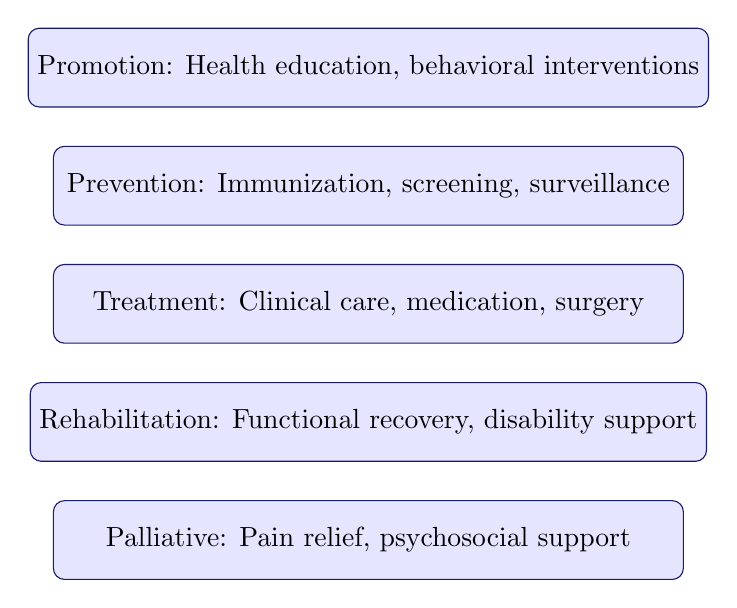
\begin{tikzpicture}[node distance=1.5cm]
\tikzstyle{dimension} = [rectangle, rounded corners, minimum width=8cm, minimum height=1cm, text centered]

\node (D1) [dimension, draw=MidnightBlue, fill=blue!10] {Promotion: Health education, behavioral interventions};
\node (D2) [dimension, below of=D1, draw=MidnightBlue, fill=blue!10] {Prevention: Immunization, screening, surveillance};
\node (D3) [dimension, below of=D2, draw=MidnightBlue, fill=blue!10] {Treatment: Clinical care, medication, surgery};
\node (D4) [dimension, below of=D3, draw=MidnightBlue, fill=blue!10] {Rehabilitation: Functional recovery, disability support};
\node (D5) [dimension, below of=D4, draw=MidnightBlue, fill=blue!10] {Palliative: Pain relief, psychosocial support};
\end{tikzpicture}
\end{center}
\end{frame}

\begin{frame}{UHC Dimensions: Financial Risk Protection}
\begin{columns}
\begin{column}{0.5\textwidth}
\begin{block}{Financial Protection Indicators}
\begin{itemize}
\item Out-of-pocket expenditure (OOP) as percentage of total health expenditure
\item Incidence of catastrophic health spending (>10\% or 25\% of household consumption)
\end{itemize}
\end{block}
\end{column}
\begin{column}{0.5\textwidth}
\begin{block}{Global Situation}
\begin{itemize}
\item 3.6 billion people lack access to essential health services
\item 100 million pushed into extreme poverty due to health costs annually
\end{itemize}
\end{block}
\end{column}
\end{columns}

\begin{block}{Key Insight}
UHC represents a balance between expanding service coverage while protecting households from financial ruin due to healthcare costs.
\end{block}
\end{frame}

\begin{frame}{UHC Dimensions: Equity and Access}
Equity considerations in UHC include:

\begin{columns}
\begin{column}{0.5\textwidth}
\begin{block}{Horizontal Equity}
\begin{itemize}
\item Equal access for equal need
\item Same services available to all populations
\end{itemize}
\end{block}
\end{column}
\begin{column}{0.5\textwidth}
\begin{block}{Vertical Equity}
\begin{itemize}
\item Greater resources for greater need
\item Priority to vulnerable populations
\end{itemize}
\end{block}
\end{column}
\end{columns}

\begin{block}{Coverage Gaps}
Significant disparities persist across:
\begin{itemize}
\item Geographic location (rural vs. urban)
\item Socioeconomic status
\item Gender and age
\end{itemize}
\end{block}
\end{frame}

\subsection{Health Informatics Tools and UHC}

\begin{frame}{Electronic Health Records and UHC}
EHRs contribute to UHC through multiple pathways:

\begin{center}
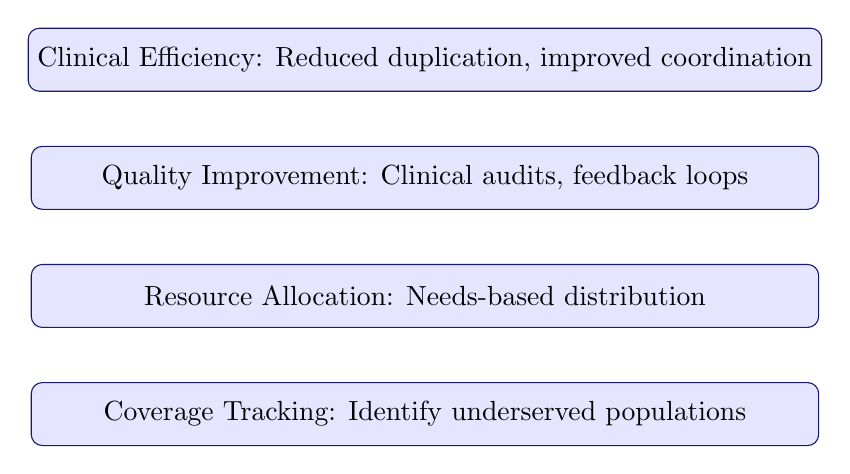
\begin{tikzpicture}[node distance=1.5cm]
\tikzstyle{pathway} = [rectangle, rounded corners, minimum width=10cm, minimum height=0.8cm, text centered]

\node (P1) [pathway, draw=MidnightBlue, fill=blue!10] {Clinical Efficiency: Reduced duplication, improved coordination};
\node (P2) [pathway, below of=P1, draw=MidnightBlue, fill=blue!10] {Quality Improvement: Clinical audits, feedback loops};
\node (P3) [pathway, below of=P2, draw=MidnightBlue, fill=blue!10] {Resource Allocation: Needs-based distribution};
\node (P4) [pathway, below of=P3, draw=MidnightBlue, fill=blue!10] {Coverage Tracking: Identify underserved populations};
\end{tikzpicture}
\end{center}
\end{frame}

\begin{frame}{Case Study: Rwanda's EHR Implementation}
Rwanda's experience demonstrates EHR contribution to UHC goals:

\begin{itemize}
\item \textbf{System}: Rwanda Health Information Exchange (RHIE) integrated with iHRIS
\item \textbf{Coverage}: 95\% of health facilities using electronic systems
\item \textbf{Outcomes}: Improved immunization coverage (from 70\% to 95\%)
\item \textbf{Equity}: Reduced urban-rural disparities in service delivery
\end{itemize}

\begin{block}{Key Lesson}
Strong government ownership, community health worker integration, and mobile connectivity enabled Rwanda's successful EHR scale-up supporting UHC progress.
\end{block}
\end{frame}

\begin{frame}{DHIS2 and Health Information Systems}
DHIS2 (District Health Information Software 2) serves as a core platform for health information in LMICs:

\begin{columns}
\begin{column}{0.5\textwidth}
\begin{block}{Key Features}
\begin{itemize}
\item Open-source platform
\item Modular and customizable
\item Offline data collection
\item Real-time dashboards
\end{itemize}
\end{block}
\end{column}
\begin{column}{0.5\textwidth}
\begin{block}{Global Adoption}
\begin{itemize}
\item 70+ countries implemented
\item 2+ billion population coverage
\item Standard for health sector reporting
\end{itemize}
\end{block}
\end{column}
\end{columns}

\begin{block}{UHC Contribution}
DHIS2 enables tracking of UHC service coverage indicators, supporting evidence-based resource allocation and performance management.
\end{block}
\end{frame}

\begin{frame}{mHealth and Telemedicine for UHC}
Mobile health technologies extend service delivery reach:

\begin{center}
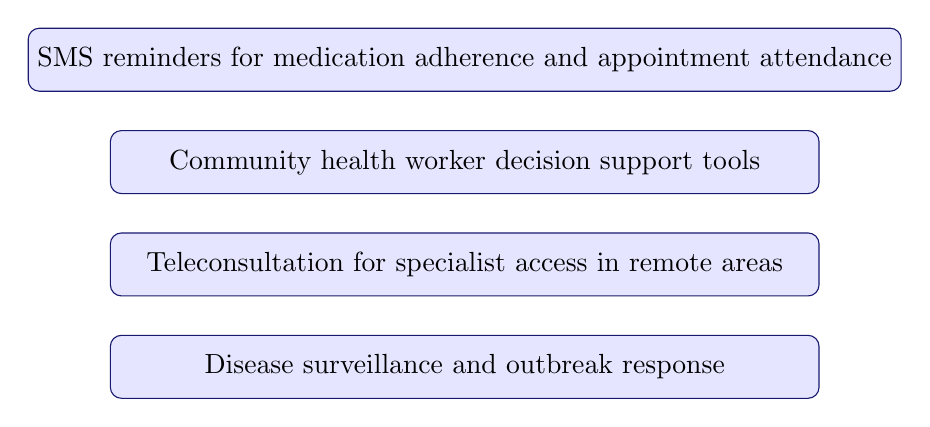
\begin{tikzpicture}[node distance=1.3cm]
\tikzstyle{application} = [rectangle, rounded corners, minimum width=9cm, minimum height=0.8cm, text centered]

\node (M1) [application, draw=MidnightBlue, fill=blue!10] {SMS reminders for medication adherence and appointment attendance};
\node (M2) [application, below of=M1, draw=MidnightBlue, fill=blue!10] {Community health worker decision support tools};
\node (M3) [application, below of=M2, draw=MidnightBlue, fill=blue!10] {Teleconsultation for specialist access in remote areas};
\node (M4) [application, below of=M3, draw=MidnightBlue, fill=blue!10] {Disease surveillance and outbreak response};
\end{tikzpicture}
\end{center}
\end{frame}

\begin{frame}{Case Study: mHero in Liberia}
The mHero (Mobile Health Worker Emergency Response) system in Liberia:

\begin{block}{Implementation}
\begin{itemize}
\item Platform: UNICEF's RapidPro
\item Launch: 2014 during Ebola outbreak
\item Coverage: 1,400+ health workers
\end{itemize}
\end{block}

\begin{block}{Outcomes}
\begin{itemize}
\item Real-time communication with health workers
\item Health facility status monitoring
\item Supply chain management support
\end{itemize}
\end{block}

\begin{block}{UHC Relevance}
mHealth demonstrates potential for strengthening health workforce communication and service delivery continuity essential for UHC.
\end{block}
\end{frame}

\begin{frame}{Digital Health Financing and Registries}
Digital systems support UHC financing mechanisms:

\begin{columns}
\begin{column}{0.5\textwidth}
\begin{block}{Health Financing Tools}
\begin{itemize}
\item Electronic claims processing
\item Payment verification systems
\item Fraud detection
\end{itemize}
\end{block}
\end{column}
\begin{column}{0.5\textwidth}
\begin{block}{Registries}
\begin{itemize}
\item Population registries
\item Health facility registries
\item Civil registration and vital statistics
\end{itemize}
\end{block}
\end{column}
\end{columns}

\begin{block}{Case Study: Ghana's NHIS}
Ghana's National Health Insurance Scheme uses smart cards and electronic claims processing, achieving near-universal coverage and reducing out-of-pocket expenditure from 40\% to 33\% of total health spending.
\end{block}
\end{frame}

\subsection{Mapping to WHO Health System Building Blocks}

\begin{frame}{Health Informatics Contributions to WHO Building Blocks}
\begin{center}
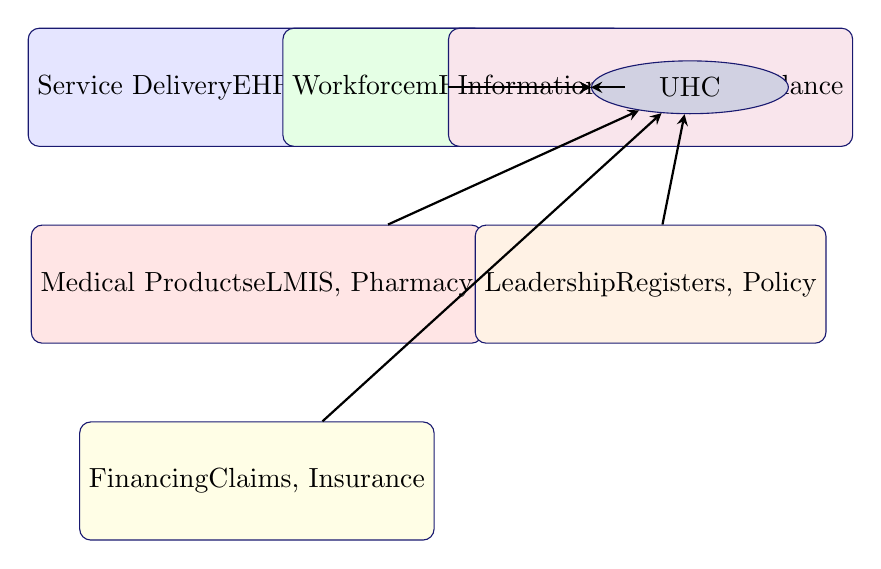
\begin{tikzpicture}[node distance=1.5cm]
\tikzstyle{block} = [rectangle, rounded corners, minimum width=4cm, minimum height=1.5cm, text centered, draw=MidnightBlue]
\tikzstyle{arrow} = [thick,->,>=stealth]

\node (service) [block, fill=blue!10] {Service Delivery\\EHRs, Telemedicine};
\node (workforce) [block, fill=green!10, right of=service, xshift=1cm] {Workforce\\mHero, Training};
\node (info) [block, fill=purple!10, right of=workforce, xshift=1cm] {Information\\DHIS2, Surveillance};
\node (products) [block, fill=red!10, below of=service, yshift=-1cm] {Medical Products\\eLMIS, Pharmacy};
\node (financing) [block, fill=yellow!10, below of=products, yshift=-1cm] {Financing\\Claims, Insurance};
\node (governance) [block, fill=orange!10, below of=info, yshift=-1cm] {Leadership\\Registers, Policy};

\node (UHC) at (5.5,0) [ellipse, draw=MidnightBlue, fill=MidnightBlue!20, minimum width=2.5cm] {UHC};

\draw [arrow] (service) -- (UHC);
\draw [arrow] (workforce) -- (UHC);
\draw [arrow] (info) -- (UHC);
\draw [arrow] (products) -- (UHC);
\draw [arrow] (financing) -- (UHC);
\draw [arrow] (governance) -- (UHC);
\end{tikzpicture}
\end{center}
\end{frame}

\begin{frame}{Cross-Cutting Informatics Contributions}
Health informatics enables cross-cutting improvements:

\begin{columns}
\begin{column}{0.5\textwidth}
\begin{block}{Efficiency}
\begin{itemize}
\item Reduced administrative burden
\item Optimized resource utilization
\item Automated reporting
\end{itemize}
\end{block}
\end{column}
\begin{column}{0.5\textwidth}
\begin{block}{Accountability}
\begin{itemize}
\item Performance monitoring
\item Transparency in resource use
\item Citizen feedback mechanisms
\end{itemize}
\end{block}
\end{column}
\end{columns}

\begin{block}{Population Health}
\begin{itemize}
\item Disease surveillance and early warning
\item Epidemiological analysis
\item Targeted intervention delivery
\end{itemize}
\end{block}
\end{frame}

\subsection{Limitation Analysis and Critical Discussion}

\begin{frame}{The Digital Divide: A Fundamental Challenge}
The digital divide threatens to undermine UHC progress:

\begin{center}
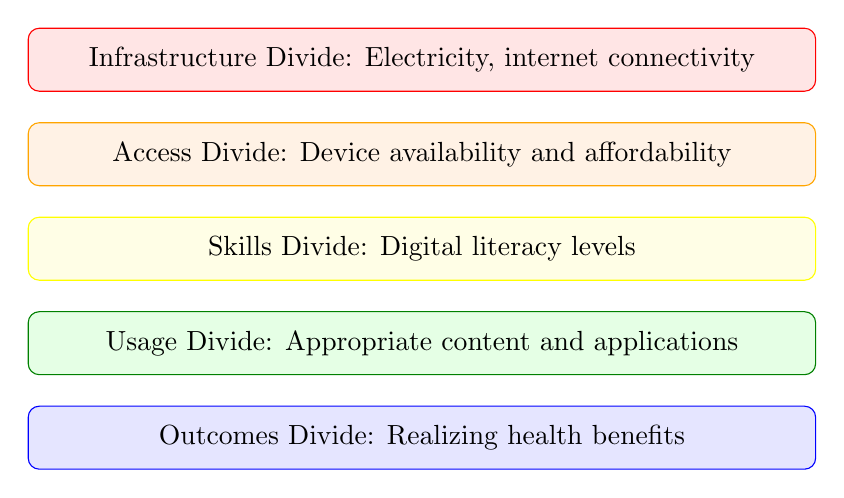
\begin{tikzpicture}[node distance=1.2cm]
\tikzstyle{divide} = [rectangle, rounded corners, minimum width=10cm, minimum height=0.8cm, text centered]

\node (D1) [divide, draw=Red, fill=red!10] {Infrastructure Divide: Electricity, internet connectivity};
\node (D2) [divide, below of=D1, draw=Orange, fill=orange!10] {Access Divide: Device availability and affordability};
\node (D3) [divide, below of=D2, draw=Yellow, fill=yellow!10] {Skills Divide: Digital literacy levels};
\node (D4) [divide, below of=D3, draw=Green, fill=green!10] {Usage Divide: Appropriate content and applications};
\node (D5) [divide, below of=D4, draw=Blue, fill=blue!10] {Outcomes Divide: Realizing health benefits};
\end{tikzpicture}
\end{center}
\end{frame}

\begin{frame}{Critical Limitations of Health Informatics for UHC}
\begin{columns}
\begin{column}{0.5\textwidth}
\begin{block}{Implementation Challenges}
\begin{itemize}
\item Sustainability beyond pilot projects
\item Integration with existing systems
\item Human capacity constraints
\end{itemize}
\end{block}
\end{column}
\begin{column}{0.5\textwidth}
\begin{block}{Equity Concerns}
\begin{itemize}
\item Risk of widening disparities
\item Gender dimensions of access
\item Urban-rural gaps
\end{itemize}
\end{block}
\end{column}
\end{columns}

\begin{block}{Evidence Gaps}
Limited rigorous evidence on health informatics cost-effectiveness for UHC in LMICs, with most studies focused on high-income country settings.
\end{block}
\end{frame}

\begin{frame}{Implementation Challenges: Real-World Examples}
\begin{center}
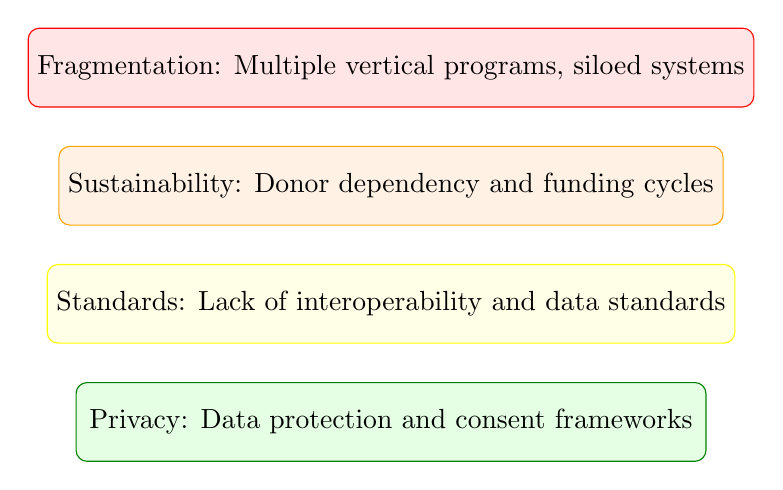
\begin{tikzpicture}[node distance=1.5cm]
\tikzstyle{challenge} = [rectangle, rounded corners, minimum width=8cm, minimum height=1cm, text centered]

\node (C1) [challenge, draw=Red, fill=red!10] {Fragmentation: Multiple vertical programs, siloed systems};
\node (C2) [challenge, below of=C1, draw=Orange, fill=orange!10] {Sustainability: Donor dependency and funding cycles};
\node (C3) [challenge, below of=C2, draw=Yellow, fill=yellow!10] {Standards: Lack of interoperability and data standards};
\node (C4) [challenge, below of=C3, draw=Green, fill=green!10] {Privacy: Data protection and consent frameworks};
\end{tikzpicture}
\end{center}
\end{frame}

\begin{frame}{Case Study: India's Digital Health Mission}
The Ayushman Bharat Digital Mission (ABDM) represents an ambitious UHC-oriented digital health transformation:

\begin{block}{Scale}
\begin{itemize}
\item Target: 1.4 billion population
\item Health ID creation for all citizens
\item Healthcare Professionals Registry
\end{itemize}
\end{block}

\begin{block}{Challenges}
\begin{itemize}
\item Privacy and consent management
\item Integration with state-level systems
\item Equity of access for marginalized populations
\end{itemize}
\end{block}

\begin{block}{Key Lesson}
Large-scale digital health initiatives require sustained political commitment, massive infrastructure investment, and robust governance frameworks to achieve UHC objectives.
\end{block}
\end{frame}

\subsection{Conclusion and Policy Implications}

\begin{frame}{Summary: Informatics for UHC}
Health informatics contributes to UHC through:

\begin{columns}
\begin{column}{0.5\textwidth}
\begin{block}{Enablers}
\begin{itemize}
\item Improved data availability and quality
\item Enhanced service delivery efficiency
\end{itemize}
\end{block}
\end{column}
\begin{column}{0.5\textwidth}
\begin{block}{Outcomes}
\begin{itemize}
\item Better resource allocation
\item Increased accountability
\end{itemize}
\end{block}
\end{column}
\end{columns}

\begin{block}{Critical Success Factors}
\begin{itemize}
\item Government leadership and ownership
\item Investment in foundational infrastructure
\item Addressing digital divides proactively
\end{itemize}
\end{block}
\end{frame}

\begin{frame}{Policy Recommendations}
\begin{columns}
\begin{column}{0.5\textwidth}
\begin{block}{Short-term}
\begin{itemize}
\item Prioritize foundational HIS strengthening
\item Build national digital health capacity
\item Establish data governance frameworks
\end{itemize}
\end{block}
\end{column}
\begin{column}{0.5\textwidth}
\begin{block}{Long-term}
\begin{itemize}
\item Sustainable domestic financing
\item Integration with UHC financing strategies
\end{itemize}
\end{block}
\end{column}
\end{columns}

\begin{block}{Research Priority}
Generate evidence on digital health interventions for UHC in LMIC contexts through rigorous implementation research and impact evaluation.
\end{block}
\end{frame}

\begin{frame}{Conclusion: Informatics and UHC}
\begin{center}
\textbf{"Digital health is not a goal in itself but a means to accelerate progress towards UHC."}
\end{center}

Key insights for MSc-level analysis:

\begin{itemize}
\item Health informatics offers significant potential but requires strategic investment
\item The digital divide threatens to undermine equity if not actively addressed
\item Sustainability depends on domestic resource mobilization and capacity building
\end{itemize}

\begin{block}{Future Outlook}
As LMICs advance towards UHC, health informatics will become increasingly central to service delivery, monitoring, and financing - but only if foundational systems and equity considerations are prioritized.
\end{block}
\end{frame}

% ============================================================================
% SECTION 3: DIGITAL TRANSFORMATION AND PATIENT-CENTERED CARE
% ============================================================================

\section{Digital Transformation and Patient-Centered Care}

\subsection{Foundations of Patient-Centered Care}

\begin{frame}{Patient-Centered Care: Definition}
Patient-centered care (PCC) is a foundational concept in healthcare quality:

\begin{block}{IOM Definition (2001)}
"Providing care that is respectful of and responsive to individual patient preferences, needs, and values, and ensuring that patient values guide all clinical decisions."
\end{block}

The Picker Institute's eight principles of patient-centered care:
\begin{enumerate}
\item Respect for patient preferences and values
\item Coordination and integration of care
\item Information, communication, and education
\item Physical comfort
\item Emotional support
\item Involvement of family and friends
\item Continuity and transition
\item Access to care
\end{enumerate}
\end{frame}

\begin{frame}{Donabedian's Quality Framework}
A. Donabedian's structure-process-outcome (SPO) model provides the foundational framework for evaluating healthcare quality:

\begin{center}
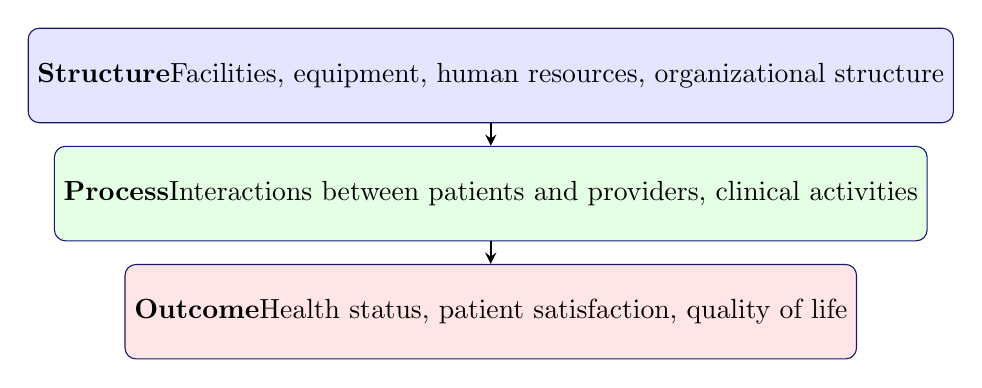
\begin{tikzpicture}[node distance=1.5cm]
\tikzstyle{element} = [rectangle, rounded corners, minimum width=5cm, minimum height=1.2cm, text centered, draw=MidnightBlue]

\node (structure) [element, fill=blue!10] {\textbf{Structure}\\[0.2cm]Facilities, equipment, human resources, organizational structure};
\node (process) [element, below of=structure, fill=green!10] {\textbf{Process}\\[0.2cm]Interactions between patients and providers, clinical activities};
\node (outcome) [element, below of=process, fill=red!10] {\textbf{Outcome}\\[0.2cm]Health status, patient satisfaction, quality of life};

\draw [thick, ->, >=stealth] (structure) -- (process);
\draw [thick, ->, >=stealth] (process) -- (outcome);
\end{tikzpicture}
\end{center}
\end{frame}

\begin{frame}{Applying Donabedian to Digital Transformation}
\begin{center}
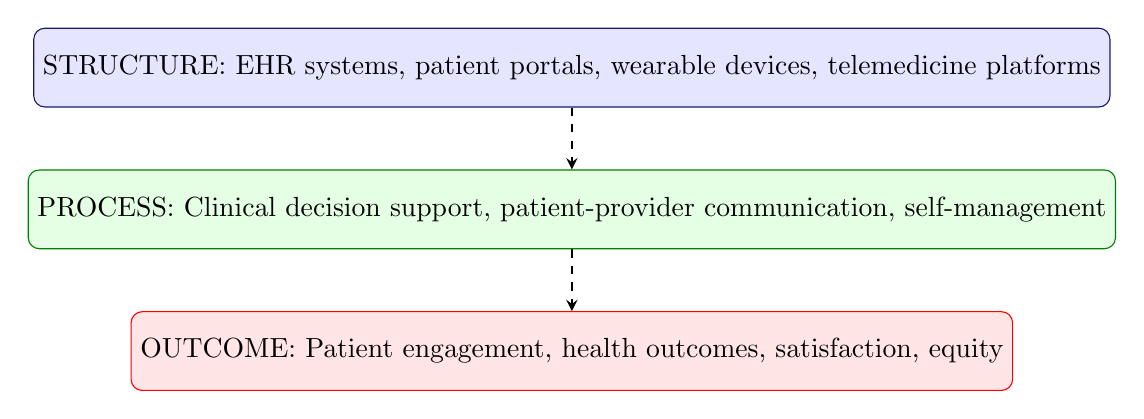
\begin{tikzpicture}[node distance=1.8cm]
\tikzstyle{level} = [rectangle, rounded corners, minimum width=10cm, minimum height=1cm, text centered]

\node (STR) [level, draw=MidnightBlue, fill=blue!10] {STRUCTURE: EHR systems, patient portals, wearable devices, telemedicine platforms};
\node (PROC) [level, below of=STR, draw=Green, fill=green!10] {PROCESS: Clinical decision support, patient-provider communication, self-management};
\node (OUT) [level, below of=PROC, draw=Red, fill=red!10] {OUTCOME: Patient engagement, health outcomes, satisfaction, equity};

\draw [thick, ->, >=stealth, dashed] (STR) -- (PROC);
\draw [thick, ->, >=stealth, dashed] (PROC) -- (OUT);
\end{tikzpicture}
\end{center}
\end{frame}

\subsection{Digital Transformation in Healthcare}

\begin{frame}{Defining Digital Transformation}
Digital transformation in healthcare refers to:

\begin{block}{Comprehensive Definition}
"The fundamental redesign of healthcare delivery through the strategic adoption of digital technologies to improve health outcomes, enhance patient experience, increase operational efficiency, and enable new models of care."
\end{block}

Key dimensions include:
\begin{itemize}
\item \textbf{Data digitization}: Paper to electronic records
\item \textbf{Connectivity}: Internet-enabled devices and platforms
\item \textbf{Automation}: AI and machine learning applications
\item \textbf{Patient empowerment}: Consumer-facing digital tools
\end{itemize}
\end{frame}

\begin{frame}{Digital Health Technology Landscape}
\begin{center}
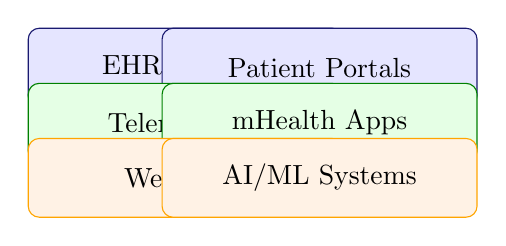
\begin{tikzpicture}[node distance=1.2cm]
\tikzstyle{tech} = [rectangle, rounded corners, minimum width=4cm, minimum height=1cm, text centered]

\node (EHR) [tech, draw=MidnightBlue, fill=blue!10] {EHR Systems};
\node (PORTAL) [tech, right of=EHR, xshift=0.5cm, draw=MidnightBlue, fill=blue!10] {Patient Portals};
\node (TELE) [tech, below of=EHR, yshift=0.5cm, draw=Green, fill=green!10] {Telemedicine};
\node (MHEALTH) [tech, right of=TELE, xshift=0.5cm, draw=Green, fill=green!10] {mHealth Apps};
\node (WEAR) [tech, below of=TELE, yshift=0.5cm, draw=Orange, fill=orange!10] {Wearables};
\node (AI) [tech, right of=WEAR, xshift=0.5cm, draw=Orange, fill=orange!10] {AI/ML Systems};
\end{tikzpicture}
\end{center}
\end{frame}

\subsection{Digital Tools and Patient-Centered Care}

\begin{frame}{Electronic Health Records and Patient Portals}
\begin{columns}
\begin{column}{0.5\textwidth}
\begin{block}{EHR Contributions to PCC}
\begin{itemize}
\item Comprehensive health history access
\item Care coordination across providers
\item Medication reconciliation
\end{itemize}
\end{block}
\end{column}
\begin{column}{0.5\textwidth}
\begin{block}{Patient Portal Features}
\begin{itemize}
\item Lab results access
\item Appointment scheduling
\item Secure messaging with providers
\end{itemize}
\end{block}
\end{column}
\end{columns}

\begin{block}{Evidence Summary}
Systematic reviews demonstrate patient portals improve patient satisfaction and medication adherence, though effects on clinical outcomes remain variable.
\end{block}
\end{frame}

\begin{frame}{Telemedicine and mHealth}
Telemedicine expands access and convenience:

\begin{center}
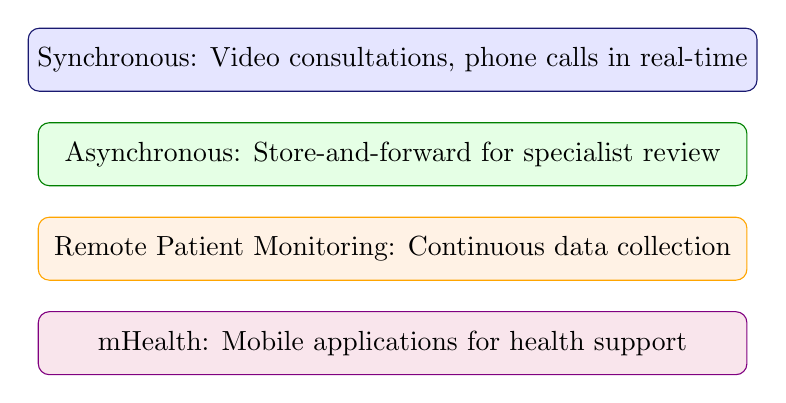
\begin{tikzpicture}[node distance=1.2cm]
\tikzstyle{modality} = [rectangle, rounded corners, minimum width=9cm, minimum height=0.8cm, text centered]

\node (T1) [modality, draw=MidnightBlue, fill=blue!10] {Synchronous: Video consultations, phone calls in real-time};
\node (T2) [modality, below of=T1, draw=Green, fill=green!10] {Asynchronous: Store-and-forward for specialist review};
\node (T3) [modality, below of=T2, draw=Orange, fill=orange!10] {Remote Patient Monitoring: Continuous data collection};
\node (T4) [modality, below of=T3, draw=Purple, fill=purple!10] {mHealth: Mobile applications for health support};
\end{tikzpicture}
\end{center}
\end{frame}

\begin{frame}{Case Study: Telemedicine in Rural India}
The eSanjeevani telemedicine platform in India:

\begin{block}{Scale}
\begin{itemize}
\item Launch: 2019, accelerated during COVID-19
\item Target: 1.4 billion population
\end{itemize}
\end{block}

\begin{block}{Impact}
\begin{itemize}
\item Over 140 million consultations completed
\item Reduced travel burden for rural patients
\item Specialist access in underserved areas
\end{itemize}
\end{block}

\begin{block}{PCC Contribution}
Telemedicine enables convenience, reduces barriers, and supports continuity of care for patients with mobility or geographic limitations.
\end{block}
\end{frame}

\begin{frame}{Wearable Devices and Remote Monitoring}
Consumer wearables and medical devices for health monitoring:

\begin{columns}
\begin{column}{0.5\textwidth}
\begin{block}{Consumer Devices}
\begin{itemize}
\item Smartwatches (heart rate, activity)
\item Fitness trackers
\item Sleep monitors
\end{itemize}
\end{block}
\end{column}
\begin{column}{0.5\textwidth}
\begin{block}{Medical Devices}
\begin{itemize}
\item Continuous glucose monitors
\item Blood pressure monitors
\item Pulse oximeters
\end{itemize}
\end{block}
\end{column}
\end{columns}

\begin{block}{PCC Implications}
Wearables enable:
\begin{itemize}
\item Continuous health data collection
\item Patient self-management
\item Early detection of health issues
\end{itemize}
\end{block}
\end{frame}

\begin{frame}{AI-Assisted Clinical Decision Support}
Artificial intelligence applications in healthcare:

\begin{center}
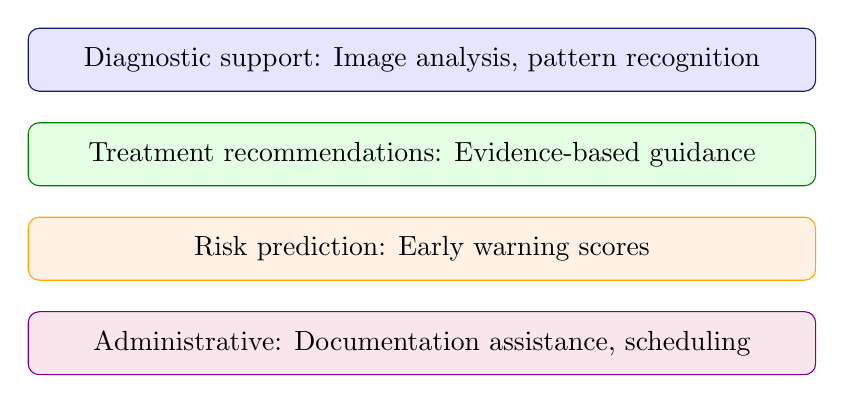
\begin{tikzpicture}[node distance=1.2cm]
\tikzstyle{application} = [rectangle, rounded corners, minimum width=10cm, minimum height=0.8cm, text centered]

\node (A1) [application, draw=MidnightBlue, fill=blue!10] {Diagnostic support: Image analysis, pattern recognition};
\node (A2) [application, below of=A1, draw=Green, fill=green!10] {Treatment recommendations: Evidence-based guidance};
\node (A3) [application, below of=A2, draw=Orange, fill=orange!10] {Risk prediction: Early warning scores};
\node (A4) [application, below of=A3, draw=Purple, fill=purple!10] {Administrative: Documentation assistance, scheduling};
\end{tikzpicture}
\end{center}
\end{frame}

\begin{frame}{Case Study: AI in Diabetic Retinopathy Screening}
IDx-DR: FDA-approved AI for autonomous diabetic retinopathy detection:

\begin{block}{Implementation}
\begin{itemize}
\item First FDA-approved autonomous AI diagnostic system
\item Non-specialist operators can perform screening
\end{itemize}
\end{block}

\begin{block}{PCC Implications}
\begin{itemize}
\item Faster diagnosis and treatment initiation
\item Reduced wait times for specialist consultations
\item Increased screening capacity in underserved areas
\end{itemize}
\end{block}

\begin{block}{Caution}
AI systems require validation, monitoring, and clear accountability frameworks to ensure patient safety.
\end{block}
\end{frame}

\subsection{Impact Analysis Using Donabedian Model}

\begin{frame}{Impact on Patient Engagement and Empowerment}
Digital tools enhance patient engagement:

\begin{center}
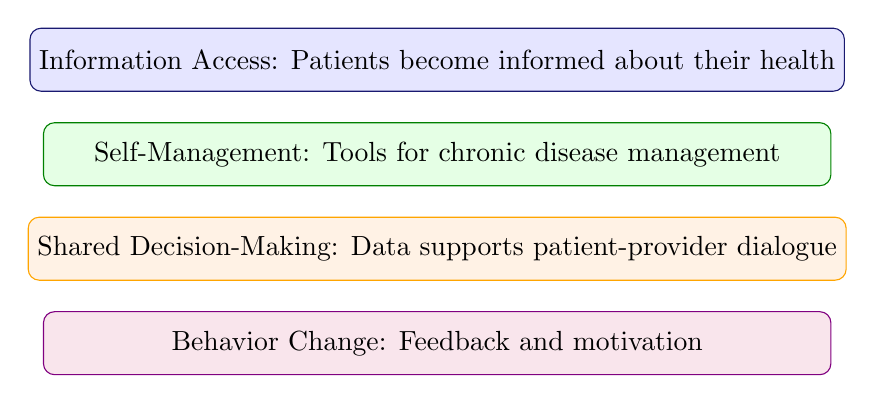
\begin{tikzpicture}[node distance=1.2cm]
\tikzstyle{level} = [rectangle, rounded corners, minimum width=10cm, minimum height=0.8cm, text centered]

\node (E1) [level, draw=MidnightBlue, fill=blue!10] {Information Access: Patients become informed about their health};
\node (E2) [level, below of=E1, draw=Green, fill=green!10] {Self-Management: Tools for chronic disease management};
\node (E3) [level, below of=E2, draw=Orange, fill=orange!10] {Shared Decision-Making: Data supports patient-provider dialogue};
\node (E4) [level, below of=E3, draw=Purple, fill=purple!10] {Behavior Change: Feedback and motivation};
\end{tikzpicture}
\end{center}
\end{frame}

\begin{frame}{Impact on Quality and Continuity of Care}
\begin{columns}
\begin{column}{0.5\textwidth}
\begin{block}{Quality Improvements}
\begin{itemize}
\item Clinical decision support reduces errors
\item Medication reconciliation improves safety
\item Care coordination tools enhance transitions
\end{itemize}
\end{block}
\end{column}
\begin{column}{0.5\textwidth]
\begin{block}{Continuity Enhancement}
\begin{itemize}
\item Unified health records across providers
\item Patient portals for ongoing communication
\item Remote monitoring for chronic conditions
\end{itemize}
\end{block}
\end{column}
\end{columns}

\begin{block}{Evidence Summary}
Digital health interventions show positive effects on process measures (medication adherence, appointment attendance) with more variable effects on clinical outcomes.
\end{block}
\end{frame}

\begin{frame}{Impact on Access and Equity}
\begin{center}
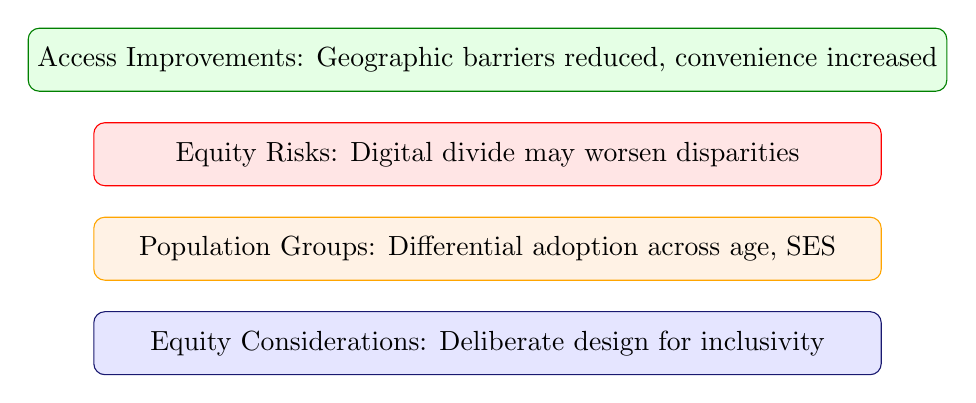
\begin{tikzpicture}[node distance=1.2cm]
\tikzstyle{impact} = [rectangle, rounded corners, minimum width=10cm, minimum height=0.8cm, text centered]

\node (I1) [impact, draw=Green, fill=green!10] {Access Improvements: Geographic barriers reduced, convenience increased};
\node (I2) [impact, below of=I1, draw=Red, fill=red!10] {Equity Risks: Digital divide may worsen disparities};
\node (I3) [impact, below of=I2, draw=Orange, fill=orange!10] {Population Groups: Differential adoption across age, SES};
\node (I4) [impact, below of=I3, draw=MidnightBlue, fill=blue!10] {Equity Considerations: Deliberate design for inclusivity};
\end{tikzpicture}
\end{center}
\end{frame}

\begin{frame}{Case Study: Rural Health App in Africa}
The WelTel mHealth intervention in Kenya:

\begin{block}{Intervention}
\begin{itemize}
\item SMS-based communication with patients
\item Focus on HIV and maternal health
\end{itemize}
\end{block}

\begin{block}{Outcomes}
\begin{itemize}
\item Improved antiretroviral therapy adherence (22\% improvement)
\item Increased facility delivery rates
\end{itemize}
\end{block}

\begin{block}{Equity Implications}
Mobile phone penetration in sub-Saharan Africa enabled reach to rural populations, though gender gaps in phone ownership remain a concern.
\end{block}
\end{frame}

\subsection{Ethical, Privacy, and Data Protection Concerns}

\begin{frame}{Ethical Considerations in Digital Health}
\begin{center}
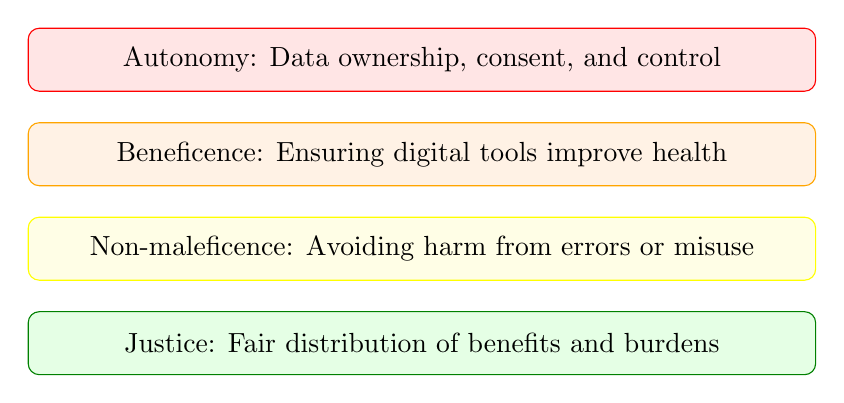
\begin{tikzpicture}[node distance=1.2cm]
\tikzstyle{ethics} = [rectangle, rounded corners, minimum width=10cm, minimum height=0.8cm, text centered]

\node (E1) [ethics, draw=Red, fill=red!10] {Autonomy: Data ownership, consent, and control};
\node (E2) [ethics, below of=E1, draw=Orange, fill=orange!10] {Beneficence: Ensuring digital tools improve health};
\node (E3) [ethics, below of=E2, draw=Yellow, fill=yellow!10] {Non-maleficence: Avoiding harm from errors or misuse};
\node (E4) [ethics, below of=E3, draw=Green, fill=green!10] {Justice: Fair distribution of benefits and burdens};
\end{tikzpicture}
\end{center}
\end{frame}

\begin{frame}{Privacy and Data Protection}
Key concerns in digital health:

\begin{columns}
\begin{column}{0.5\textwidth}
\begin{block}{Data Security Risks}
\begin{itemize}
\item Unauthorized access to health records
\item Data breaches and cyberattacks
\item Third-party data sharing
\end{itemize}
\end{block}
\end{column}
\begin{column}{0.5\textwidth}
\begin{block}{Privacy Challenges}
\begin{itemize}
\item Re-identification from de-identified data
\item Surveillance concerns
\item Cross-border data transfers
\end{itemize}
\end{block}
\end{column}
\end{columns}

\begin{block}{Regulatory Frameworks}
GDPR (EU), HIPAA (US), and emerging LMIC data protection laws establish requirements for health data handling.
\end{block}
\end{frame}

\begin{frame}{Case Study: Data Governance in AI Applications}
The Google DeepMind NHS controversy:

\begin{block}{Context}
\begin{itemize}
\item AI application for acute kidney injury detection
\item Data access through Royal Free NHS Trust
\end{itemize}
\end{block}

\begin{block}{Concerns}
\begin{itemize}
\item Insufficient patient consent for data use
\item Scope creep beyond original purpose
\end{itemize}
\end{block}

\begin{block}{Lessons}
Strong governance frameworks, transparent data use policies, and meaningful patient consent are essential for maintaining trust in digital health.
\end{block}
\end{frame}

\begin{frame}{Bias and Fairness in Digital Health}
Algorithmic bias risks in AI-driven healthcare:

\begin{center}
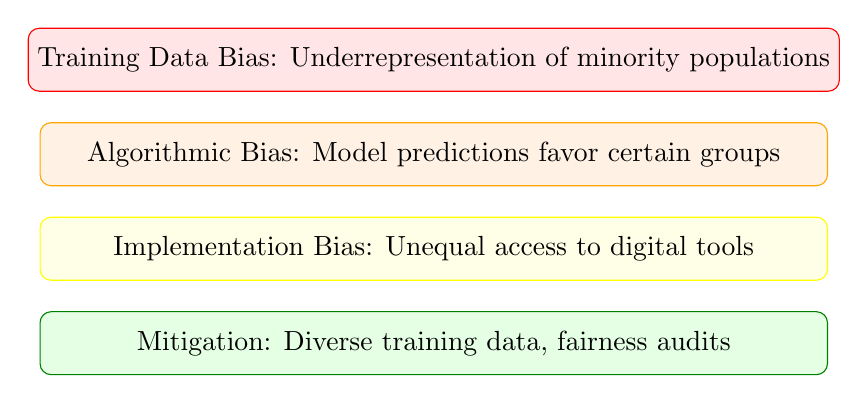
\begin{tikzpicture}[node distance=1.2cm]
\tikzstyle{risk} = [rectangle, rounded corners, minimum width=10cm, minimum height=0.8cm, text centered]

\node (B1) [risk, draw=Red, fill=red!10] {Training Data Bias: Underrepresentation of minority populations};
\node (B2) [risk, below of=B1, draw=Orange, fill=orange!10] {Algorithmic Bias: Model predictions favor certain groups};
\node (B3) [risk, below of=B2, draw=Yellow, fill=yellow!10] {Implementation Bias: Unequal access to digital tools};
\node (B4) [risk, below of=B3, draw=Green, fill=green!10] {Mitigation: Diverse training data, fairness audits};
\end{tikzpicture}
\end{center}
\end{frame}

\begin{frame}{Case Study: Racial Bias in Healthcare Algorithms}
The 2019 Science study on commercial algorithm bias:

\begin{block}{Finding}
A widely used healthcare algorithm exhibited racial bias, assigning lower risk scores to Black patients with equivalent health needs to White patients.
\end{block}

\begin{block}{Root Cause}
The algorithm used healthcare costs as a proxy for health needs, reflecting historical inequities in healthcare access.
\end{block}

\begin{block}{Implications}
Careful validation, bias testing, and ongoing monitoring are essential for AI systems in healthcare to ensure equitable outcomes.
\end{block}
\end{frame}

\subsection{Conclusion: Balancing Benefits and Risks}

\begin{frame}{Summary: Digital Transformation for PCC}
\begin{center}
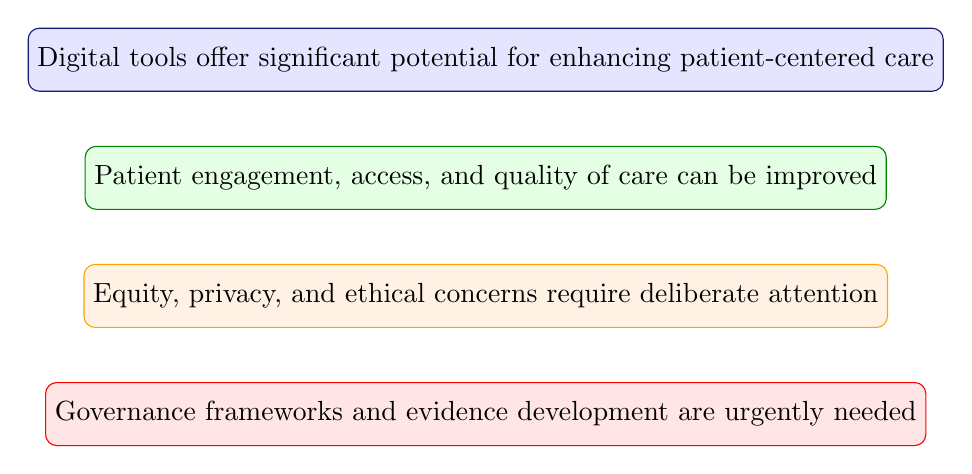
\begin{tikzpicture}[node distance=1.5cm]
\tikzstyle{summary} = [rectangle, rounded corners, minimum width=10cm, minimum height=0.8cm, text centered]

\node (S1) [summary, draw=MidnightBlue, fill=blue!10] {Digital tools offer significant potential for enhancing patient-centered care};
\node (S2) [summary, below of=S1, draw=Green, fill=green!10] {Patient engagement, access, and quality of care can be improved};
\node (S3) [summary, below of=S2, draw=Orange, fill=orange!10] {Equity, privacy, and ethical concerns require deliberate attention};
\node (S4) [summary, below of=S3, draw=Red, fill=red!10] {Governance frameworks and evidence development are urgently needed};
\end{tikzpicture}
\end{center}
\end{frame}

\begin{frame}{Conclusion: Benefits and Risks}
\begin{columns}
\begin{column}{0.5\textwidth}
\begin{block}{Benefits}
\begin{itemize}
\item Enhanced patient engagement
\item Improved access to care
\item Better informed clinical decisions
\item Continuous health monitoring
\end{itemize}
\end{block}
\end{column}
\begin{column}{0.5\textwidth}
\begin{block}{Risks}
\begin{itemize}
\item Privacy violations
\item Digital divide and inequities
\item Algorithmic bias
\end{itemize}
\end{block}
\end{column}
\end{columns}

\begin{block}{Balanced Assessment}
Digital transformation offers powerful tools for patient-centered care but requires:
\begin{itemize}
\item Robust governance
\end{itemize}
\end{block}
\end{frame}

\begin{frame}{Future Directions}
\begin{columns}
\begin{column}{0.5\textwidth}
\begin{block}{Clinical Practice}
\begin{itemize}
\item Integration of digital tools into care workflows
\item Training for digital literacy
\end{itemize}
\end{block}
\end{column}
\begin{column}{0.5\textwidth]
\begin{block}{Policy}
\begin{itemize}
\item Data protection regulations
\item Interoperability standards
\end{itemize}
\end{block}
\end{column}
\end{columns}

\begin{block}{Research}
Rigorous evaluation of digital health interventions, particularly on health outcomes and equity, is essential to guide evidence-based implementation.
\end{block}
\end{frame}

\begin{frame}{Final Remarks: Digital Transformation and PCC}
\begin{center}
\textbf{"The promise of digital health for patient-centered care can only be realized if we actively address equity, privacy, and governance challenges."}
\end{center}

Key considerations for the MSc-level analyst:
\begin{itemize}
\item Digital tools are means, not ends, for PCC
\item Context matters in implementation
\item Continuous evaluation is essential
\end{itemize}
\end{frame}

% ============================================================================
% SECTION 4: INTEROPERABILITY IN NATIONAL HEALTH INFORMATION SYSTEMS
% ============================================================================

\section{Interoperability in National Health Information Systems}

\subsection{Defining Interoperability}

\begin{frame}{Interoperability: Definition}
Interoperability in health information systems is defined as:

\begin{block}{HIMSS Definition}
"The ability of different information systems, devices and applications (or components) to access, exchange, integrate and cooperatively use data in order to ensure that the information is usable in the intended manner."
\end{block}

A more comprehensive definition by ISO/IEEE 11073 emphasizes:
\begin{itemize}
\item \textbf{Technical} compatibility between systems
\item \textbf{Semantic} understanding of exchanged data
\item \textbf{Organizational} alignment and workflow integration
\end{itemize}
\end{frame}

\begin{frame}{Levels of Interoperability}
\begin{center}
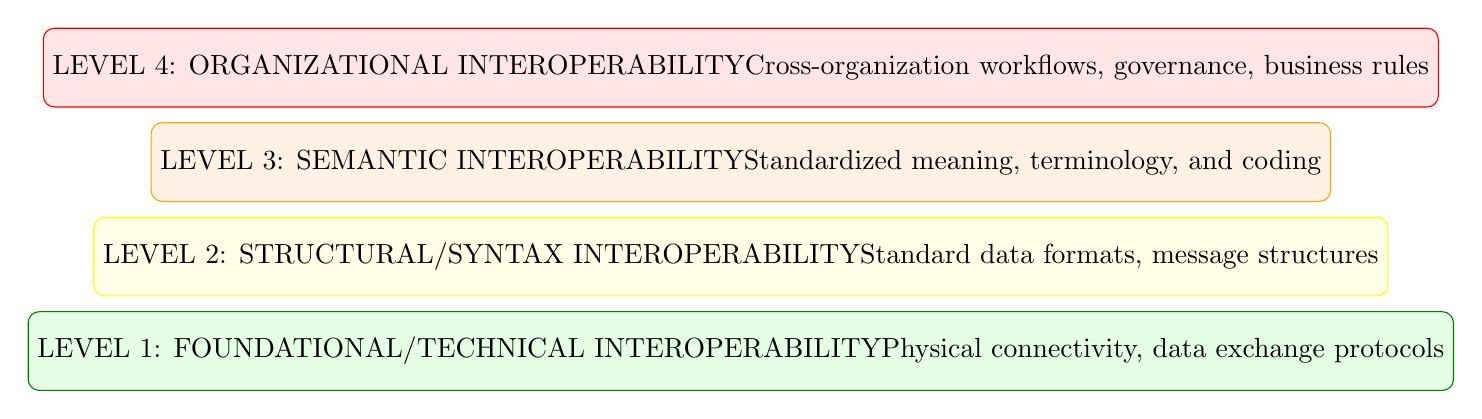
\begin{tikzpicture}[node distance=1.2cm]
\tikzstyle{level} = [rectangle, rounded corners, minimum width=10cm, minimum height=1cm, text centered]

\node (L1) [level, draw=Red, fill=red!10] {LEVEL 4: ORGANIZATIONAL INTEROPERABILITY\\
Cross-organization workflows, governance, business rules};
\node (L2) [level, below of=L1, draw=Orange, fill=orange!10] {LEVEL 3: SEMANTIC INTEROPERABILITY\\
Standardized meaning, terminology, and coding};
\node (L3) [level, below of=L2, draw=Yellow, fill=yellow!10] {LEVEL 2: STRUCTURAL/SYNTAX INTEROPERABILITY\\
Standard data formats, message structures};
\node (L4) [level, below of=L3, draw=Green, fill=green!10] {LEVEL 1: FOUNDATIONAL/TECHNICAL INTEROPERABILITY\\
Physical connectivity, data exchange protocols};
\end{tikzpicture}
\end{center}
\end{frame}

\begin{frame}{Foundational (Technical) Interoperability}
The most basic level of interoperability:

\begin{block}{Key Components}
\begin{itemize}
\item Network connectivity between systems
\item Data transmission protocols (HL7, DICOM)
\item Interface standards and APIs
\end{itemize}
\end{block}

\begin{block}{Example Technologies}
\begin{itemize}
\item VPN connections between facilities
\item HL7 messaging for lab results
\item REST APIs for application integration
\end{itemize}
\end{block}

\begin{block}{Limitation}
Technical interoperability alone does not ensure that systems can interpret the exchanged data meaningfully.
\end{block}
\end{frame}

\begin{frame}{Structural (Syntactic) Interoperability}
Defines the format and structure of data exchange:

\begin{center}
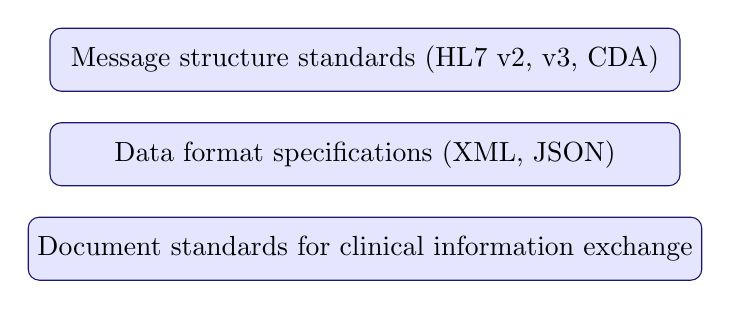
\begin{tikzpicture}[node distance=1.2cm]
\tikzstyle{element} = [rectangle, rounded corners, minimum width=8cm, minimum height=0.8cm, text centered]

\node (S1) [element, draw=MidnightBlue, fill=blue!10] {Message structure standards (HL7 v2, v3, CDA)};
\node (S2) [element, below of=S1, draw=MidnightBlue, fill=blue!10] {Data format specifications (XML, JSON)};
\node (S3) [element, below of=S2, draw=MidnightBlue, fill=blue!10] {Document standards for clinical information exchange};
\end{tikzpicture}
\end{center}
\end{frame}

\begin{frame}{Semantic Interoperability}
The highest level of meaningful data exchange:

\begin{block}{Key Elements}
\begin{itemize}
\item Standardized terminology systems
\item Consistent code mappings
\item Shared understanding of clinical concepts
\end{itemize}
\end{block}

\begin{columns}
\begin{column}{0.5\textwidth}
\begin{block}{Terminology Standards}
\begin{itemize}
\item ICD-10 (diagnoses)
\item SNOMED CT (clinical terms)
\item LOINC (laboratory)
\end{itemize}
\end{block}
\end{column}
\begin{column}{0.5\textwidth}
\begin{block}{Code Systems}
\begin{itemize}
\item RxNorm (medications)
\item CPT (procedures)
\item ATC (drugs)
\end{itemize}
\end{block}
\end{column}
\end{columns}

\begin{block}{Goal}
Ensures that receiving systems interpret data exactly as the sending system intended.
\end{block}
\end{frame}

\begin{frame}{Organizational Interoperability}
Addresses the human and process dimensions:

\begin{center}
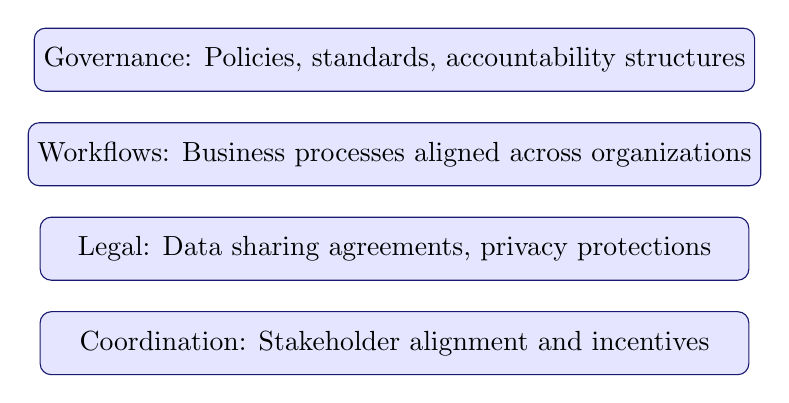
\begin{tikzpicture}[node distance=1.2cm]
\tikzstyle{element} = [rectangle, rounded corners, minimum width=9cm, minimum height=0.8cm, text centered]

\node (O1) [element, draw=MidnightBlue, fill=blue!10] {Governance: Policies, standards, accountability structures};
\node (O2) [element, below of=O1, draw=MidnightBlue, fill=blue!10] {Workflows: Business processes aligned across organizations};
\node (O3) [element, below of=O2, draw=MidnightBlue, fill=blue!10] {Legal: Data sharing agreements, privacy protections};
\node (O4) [element, below of=O3, draw=MidnightBlue, fill=blue!10] {Coordination: Stakeholder alignment and incentives};
\end{tikzpicture}
\end{center}
\end{frame}

\subsection{Challenges to Interoperability}

\begin{frame}{Fragmented Systems and Legacy Platforms}
Health information system fragmentation is a pervasive challenge:

\begin{columns}
\begin{column}{0.5\textwidth}
\begin{block}{Fragmentation Sources}
\begin{itemize}
\item Vertical disease programs (HIV, TB, malaria)
\item Multiple donor-funded systems
\item Parallel public and private systems
\end{itemize}
\end{block}
\end{column}
\begin{column}{0.5\textwidth]
\begin{block}{Legacy System Issues}
\begin{itemize}
\item Outdated technology stacks
\item Limited integration capabilities
\item High migration costs
\end{itemize}
\end{block}
\end{column}
\end{columns}

\begin{block}{Case Example: Kenya's HIS Landscape}
Over 40 distinct digital health systems operate in Kenya, including DHIS2, KenyaEMR, Afya-app, and multiple donor-funded platforms, creating significant integration challenges.
\end{block}
\end{frame}

\begin{frame}{Lack of Standards Adoption}
Despite existence of standards, adoption remains limited:

\begin{center}
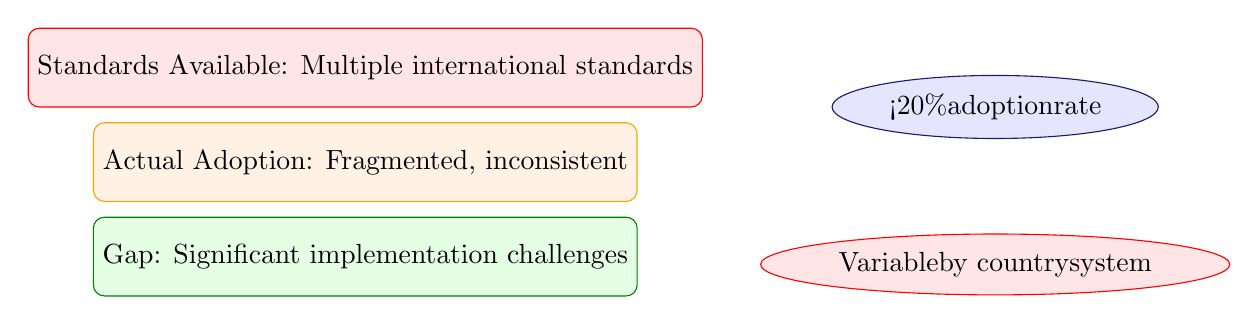
\begin{tikzpicture}[node distance=1.2cm]
\tikzstyle{bar} = [rectangle, rounded corners, minimum width=6cm, minimum height=1cm, text centered]

\node (ADOPT) [bar, draw=Red, fill=red!10] {Standards Available: Multiple international standards};
\node (ACTUAL) [bar, below of=ADOPT, draw=Orange, fill=orange!10] {Actual Adoption: Fragmented, inconsistent};
\node (GAP) [bar, below of=ACTUAL, draw=Green, fill=green!10] {Gap: Significant implementation challenges};

\node (percent) at (8,-0.5) [ellipse, draw=MidnightBlue, fill=blue!10] {<20\%\\adoption\\rate};
\node (percent2) at (8,-2.5) [ellipse, draw=Red, fill=red!10] {Variable\\by country\\system};
\end{tikzpicture}
\end{center}
\end{frame}

\begin{frame}{Standards Reference Guide}
\begin{center}
\begin{tabular}{p{3cm}p{4cm}p{4cm}}
\toprule
\textbf{Standard} & \textbf{Purpose} & \textbf{Adoption Status} \\
\midrule
HL7 v2.x & Messaging (legacy) & Widely adopted globally \\
HL7 CDA & Clinical documents & Moderate adoption \\
HL7 FHIR & Modern web APIs & Growing rapidly \\
DICOM & Medical imaging & Standard in radiology \\
IHE Profiles & Integration profiles & Limited adoption \\
\bottomrule
\end{tabular}
\end{center}
\end{frame}

\begin{frame}{Governance and Policy Gaps}
Many countries lack adequate governance frameworks:

\begin{center}
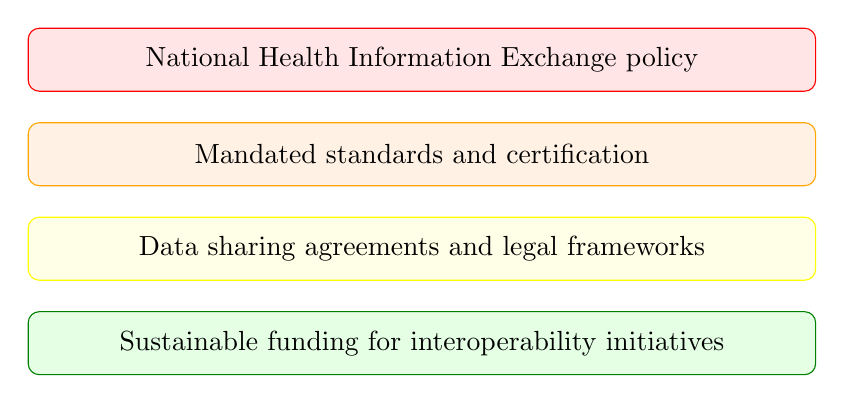
\begin{tikzpicture}[node distance=1.2cm]
\tikzstyle{gap} = [rectangle, rounded corners, minimum width=10cm, minimum height=0.8cm, text centered]

\node (G1) [gap, draw=Red, fill=red!10] {National Health Information Exchange policy};
\node (G2) [gap, below of=G1, draw=Orange, fill=orange!10] {Mandated standards and certification};
\node (G3) [gap, below of=G2, draw=Yellow, fill=yellow!10] {Data sharing agreements and legal frameworks};
\node (G4) [gap, below of=G3, draw=Green, fill=green!10] {Sustainable funding for interoperability initiatives};
\end{tikzpicture}
\end{center}
\end{frame}

\begin{frame}{Data Quality and Privacy Issues}
\begin{columns}
\begin{column}{0.5\textwidth}
\begin{block}{Data Quality Challenges}
\begin{itemize}
\item Inconsistent data entry practices
\item Missing and erroneous data
\item Non-standardized coding
\end{itemize}
\end{block}
\end{column}
\begin{column}{0.5\textwidth}
\begin{block}{Privacy Concerns}
\begin{itemize}
\item Consent management across systems
\item Data minimization principles
\item Cross-border data flows
\end{itemize}
\end{block}
\end{column}
\end{columns}

\begin{block}{Key Insight}
Poor data quality at source undermines all interoperability efforts, as exchanging bad data merely propagates errors.
\end{block}
\end{frame}

\begin{frame}{Human Capacity Limitations}
Workforce constraints impede interoperability:

\begin{center}
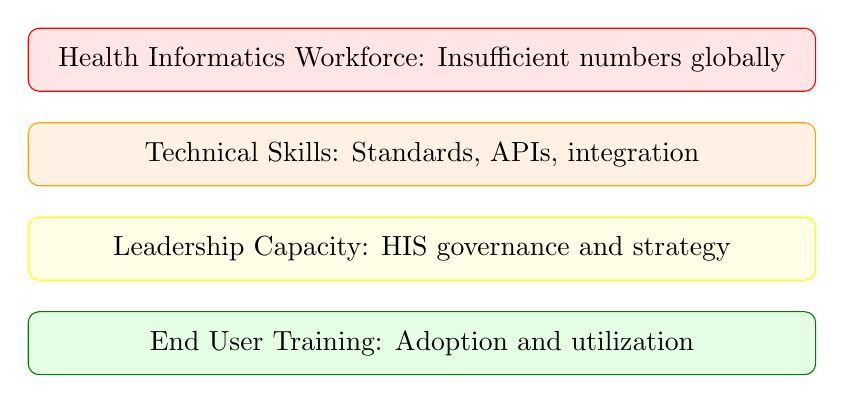
\begin{tikzpicture}[node distance=1.2cm]
\tikzstyle{capacity} = [rectangle, rounded corners, minimum width=10cm, minimum height=0.8cm, text centered]

\node (C1) [capacity, draw=Red, fill=red!10] {Health Informatics Workforce: Insufficient numbers globally};
\node (C2) [capacity, below of=C1, draw=Orange, fill=orange!10] {Technical Skills: Standards, APIs, integration};
\node (C3) [capacity, below of=C2, draw=Yellow, fill=yellow!10] {Leadership Capacity: HIS governance and strategy};
\node (C4) [capacity, below of=C3, draw=Green, fill=green!10] {End User Training: Adoption and utilization};
\end{tikzpicture}
\end{center}
\end{frame}

\begin{frame}{Case Study: Australia's My Health Record}
Australia's national EHR system provides lessons on interoperability:

\begin{block}{Implementation}
\begin{itemize}
\item Launched 2012, opt-out model from 2018
\item 23+ million registered records
\end{itemize}
\end{block}

\begin{block}{Achievements}
\begin{itemize}
\item Prescription dispensing integration
\item Pathology and imaging reports
\end{itemize}
\end{block}

\begin{block}{Challenges}
\begin{itemize}
\item Limited clinical document upload rates
\item Provider system integration complexity
\end{itemize}
\end{block}
\end{frame}

\begin{frame}{Case Study: India's ABDM Ecosystem}
India's Ayushman Bharat Digital Mission represents an ambitious interoperability framework:

\begin{block}{Architecture Components}
\begin{itemize}
\item Health ID for patient identification
\item Healthcare Professionals Registry (HPR)
\item Health Facility Registry (HFR)
\end{itemize}
\end{block}

\begin{block}{Interoperability Features}
\begin{itemize}
\item Unified Health Interface (UHI) for exchange
\item National Health Claims Exchange
\end{itemize}
\end{block}

\begin{block}{Challenges}
\begin{itemize}
\item Scale and diversity of health sector
\end{itemize}
\end{block}
\end{frame}

\subsection{Implications for Health System Performance}

\begin{frame}{Impact on Continuity of Care}
Interoperability directly affects care quality:

\begin{center}
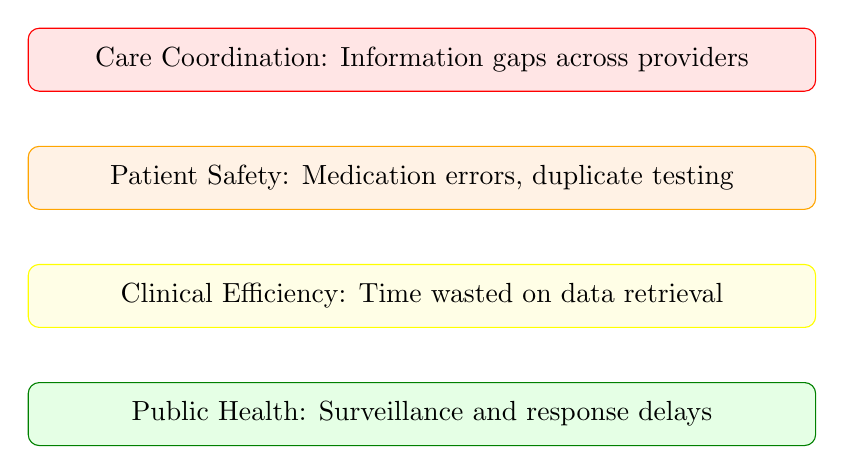
\begin{tikzpicture}[node distance=1.5cm]
\tikzstyle{impact} = [rectangle, rounded corners, minimum width=10cm, minimum height=0.8cm, text centered]

\node (I1) [impact, draw=Red, fill=red!10] {Care Coordination: Information gaps across providers};
\node (I2) [impact, below of=I1, draw=Orange, fill=orange!10] {Patient Safety: Medication errors, duplicate testing};
\node (I3) [impact, below of=I2, draw=Yellow, fill=yellow!10] {Clinical Efficiency: Time wasted on data retrieval};
\node (I4) [impact, below of=I3, draw=Green, fill=green!10] {Public Health: Surveillance and response delays};
\end{tikzpicture}
\end{center}
\end{frame}

\begin{frame}{Impact on Health System Performance}
\begin{columns}
\begin{column}{0.5\textwidth}
\begin{block}{Individual Patient Level}
\begin{itemize}
\item Better informed clinical decisions
\item Reduced duplicate testing
\item Seamless referrals
\end{itemize}
\end{block}
\end{column}
\begin{column}{0.5\textwidth}
\begin{block}{System Level}
\begin{itemize}
\item Population health management
\item Resource allocation efficiency
\item Quality measurement and improvement
\end{itemize}
\end{block}
\end{column}
\end{columns}

\begin{block}{Economic Impact}
Studies estimate that full interoperability could save healthcare systems \$30-\$150 billion annually through reduced duplication, improved efficiency, and better outcomes.
\end{block}
\end{frame}

\begin{frame}{Case Study: HIV Care Cascade in South Africa}
The eThekwini district HIV program demonstrates interoperability importance:

\begin{block}{Challenge}
\begin{itemize}
\item Multiple parallel systems: Tier.net, TIER.Health, DHIS2
\end{itemize}
\end{block}

\begin{block}{Impact}
\begin{itemize}
\item Difficulty tracking patients across facilities
\item Incomplete reporting for PEPFAR indicators
\end{itemize}
\end{block}

\begin{block}{Solution}
Integration layer to standardize data exchange between systems, improving care continuity and reporting accuracy.
\end{block}
\end{frame}

\subsection{Recommendations for Strengthening Interoperability}

\begin{frame}{Strategic Recommendations}
\begin{center}
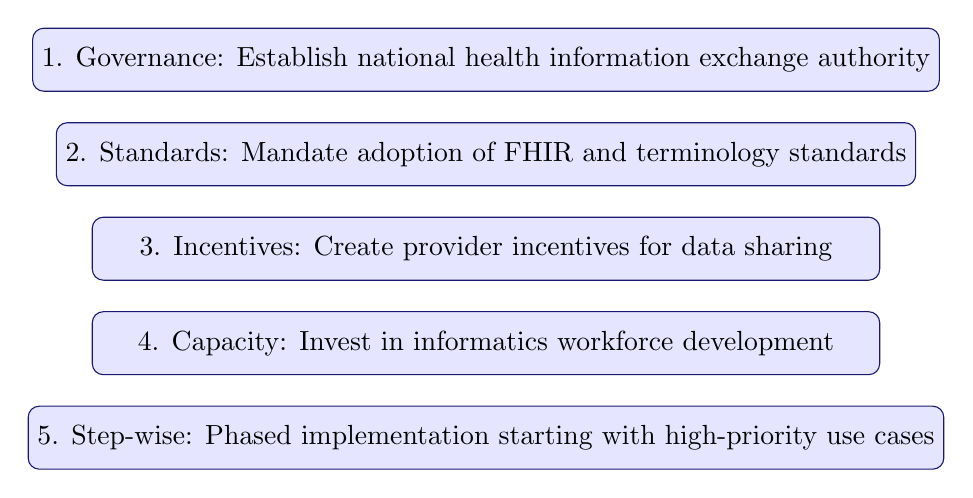
\begin{tikzpicture}[node distance=1.2cm]
\tikzstyle{rec} = [rectangle, rounded corners, minimum width=10cm, minimum height=0.8cm, text centered]

\node (R1) [rec, draw=MidnightBlue, fill=blue!10] {1. Governance: Establish national health information exchange authority};
\node (R2) [rec, below of=R1, draw=MidnightBlue, fill=blue!10] {2. Standards: Mandate adoption of FHIR and terminology standards};
\node (R3) [rec, below of=R2, draw=MidnightBlue, fill=blue!10] {3. Incentives: Create provider incentives for data sharing};
\node (R4) [rec, below of=R3, draw=MidnightBlue, fill=blue!10] {4. Capacity: Invest in informatics workforce development};
\node (R5) [rec, below of=R4, draw=MidnightBlue, fill=blue!10] {5. Step-wise: Phased implementation starting with high-priority use cases};
\end{tikzpicture}
\end{center}
\end{frame}

\begin{frame}{Technical Implementation Recommendations}
\begin{columns}
\begin{column}{0.5\textwidth}
\begin{block}{Standards-Based Approach}
\begin{itemize}
\item Adopt HL7 FHIR as primary standard
\item Implement terminology standardization (SNOMED CT, ICD-11, LOINC)
\end{itemize}
\end{block}
\end{column}
\begin{column}{0.5\textwidth]
\begin{block}{Integration Architecture}
\begin{itemize}
\item API-first design principles
\item Enterprise service bus or integration engine
\end{itemize}
\end{block}
\end{column}
\end{columns}

\begin{block}{LMIC Considerations}
Open-source solutions (OpenHIM, OpenMRS) and regional initiatives (Africa Health Information Highway) offer context-appropriate options.
\end{block}
\end{frame}

\begin{frame}{Case Study: New Zealand's HISO Standards}
New Zealand provides an example of coordinated standards adoption:

\begin{block}{Approach}
\begin{itemize}
\item Health Information Standards Organization (HISO)
\item Mandated FHIR adoption for new systems
\item National terminology services
\end{itemize}
\end{block}

\begin{block}{Outcomes}
\begin{itemize}
\item 98\% of primary care using standards-compliant EHRs
\item Integrated with national health information exchange
\end{itemize}
\end{block}

\begin{block}{Transferable Lessons}
Political commitment, dedicated standards body, and phased implementation approach enabled New Zealand's progress.
\end{block}
\end{frame}

\begin{frame}{Conclusion: Interoperability for Health Systems}
Interoperability is essential for:

\begin{itemize}
\item \textbf{Continuity of care} across providers and settings
\item \textbf{Health system efficiency} through reduced duplication
\item \textbf{Population health management} through data integration
\item \textbf{Universal Health Coverage} through equitable service delivery
\end{itemize}

\begin{block}{Final Assessment}
Achieving interoperability requires sustained commitment to governance, standards adoption, capacity building, and technical infrastructure - but the benefits for health system performance are substantial.
\end{block}
\end{frame}

% ============================================================================
% FINAL SECTION: CONCLUSIONS AND FUTURE DIRECTIONS
% ============================================================================

\section{Synthesis and Future Directions}

\begin{frame}{Cross-Cutting Themes}
The four presentations reveal interconnected themes:

\begin{center}
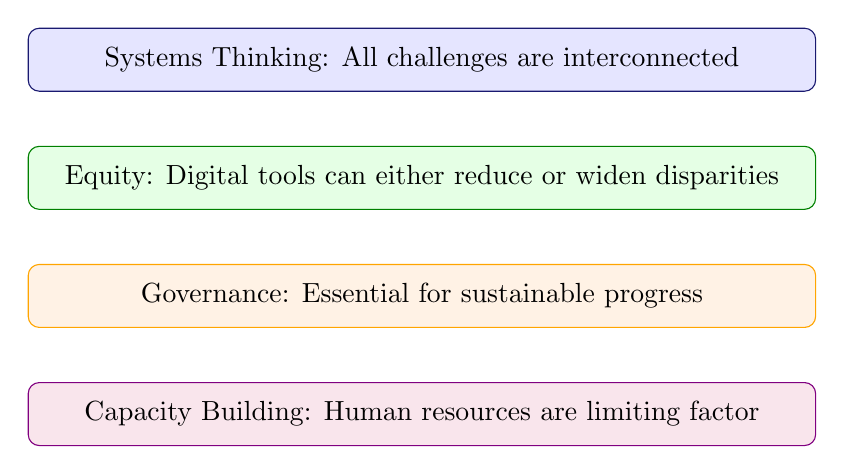
\begin{tikzpicture}[node distance=1.5cm]
\tikzstyle{theme} = [rectangle, rounded corners, minimum width=10cm, minimum height=0.8cm, text centered]

\node (T1) [theme, draw=MidnightBlue, fill=blue!10] {Systems Thinking: All challenges are interconnected};
\node (T2) [theme, below of=T1, draw=Green, fill=green!10] {Equity: Digital tools can either reduce or widen disparities};
\node (T3) [theme, below of=T2, draw=Orange, fill=orange!10] {Governance: Essential for sustainable progress};
\node (T4) [theme, below of=T3, draw=Purple, fill=purple!10] {Capacity Building: Human resources are limiting factor};
\end{tikzpicture}
\end{center}
\end{frame}

\begin{frame}{Implications for Public Health Practice}
\begin{columns}
\begin{column}{0.5\textwidth}
\begin{block}{Policy Implications}
\begin{itemize}
\item Strategic investment in digital health infrastructure
\item Development of national digital health strategies
\end{itemize}
\end{block}
\end{column}
\begin{column}{0.5\textwidth]
\begin{block}{Practice Implications}
\begin{itemize}
\item Integration of informatics into public health training
\end{itemize}
\end{block}
\end{column}
\end{columns}

\begin{block}{Research Priorities}
Evidence generation on digital health interventions in LMIC contexts, development of context-appropriate solutions, and rigorous evaluation frameworks.
\end{block}
\end{frame}

\begin{frame}{Future Trends in Health Informatics}
Emerging developments shaping the field:

\begin{columns}
\begin{column}{0.5\textwidth}
\begin{block}{Technological}
\begin{itemize}
\item Artificial intelligence and machine learning
\item Blockchain for data integrity
\item Internet of Medical Things (IoMT)
\end{itemize}
\end{block}
\end{column}
\begin{column}{0.5\textwidth]
\begin{block}{Policy}
\begin{itemize}
\item Global digital health strategies
\end{itemize}
\end{block}
\end{column}
\end{columns}

\begin{block}{Ethical}
\begin{itemize}
\item Algorithmic fairness and bias mitigation
\end{itemize}
\end{block}
\end{frame}

\begin{frame}{Final Synthesis}
\begin{center}
\textbf{"Health informatics offers transformative potential for health systems, but realizing this potential requires addressing fundamental challenges of infrastructure, capacity, governance, and equity."}
\end{center}

Key take-home messages for the MSc analyst:

\begin{itemize}
\item Apply systems thinking to understand interconnected challenges
\item Prioritize equity in all digital health initiatives
\item Build sustainable domestic capacity beyond donor funding
\end{itemize}

\begin{block}{Closing Remark}
As we advance towards Universal Health Coverage, health informatics will be increasingly central to improving health outcomes - but only if we approach it with strategic vision, evidence-based implementation, and commitment to equity.
\end{block}
\end{frame}

\begin{frame}{References}
\begin{small}
\begin{itemize}
\item World Health Organization. (2016). Global strategy on digital health 2020-2025.
\item World Health Organization. (2010). Monitoring the building blocks of health systems.
\item HIMSS. (2023). Interoperability in healthcare.
\item Donabedian, A. (2003). The quality of care: How can it be assessed?
\item Institute of Medicine. (2001). Crossing the quality chasm.
\item Bahri, S. (2020). Telehealth for universal health coverage.
\item Kruse, C.S., et al. (2017). Telehealth and patient satisfaction.
\item European Commission. (2023). Ethics guidelines for trustworthy AI.
\end{itemize}
\end{small}
\end{frame}

\end{document}
